\section{Resultados e discuss\~ao}\label{sec:resultados}

% Configurações dos Exemplos 2 e 3 conferidas com durability/01--05.
% As marcações \falta identificam resultados ainda dependentes da execução.

Os exemplos numéricos examinam três questões complementares: a capacidade de representar uma distribuição de resposta que evolui no tempo, a aplicação dessa representação à durabilidade do concreto armado e o efeito de uma política preventiva sobre o tempo disponível para intervir. Após a verificação isolada do ajuste da GLD, o Exemplo~1 utiliza um problema idealizado de resistência e solicitação, cuja simplicidade permite comparar o emulador com a simulação direta. O Exemplo~2 considera a margem entre o cobrimento e a profundidade carbonatada, incorporando a variabilidade do material, do cobrimento e da umidade relativa. O Exemplo~3 retoma o mesmo elemento e compara limiares de intervenção, interpretados como diferentes margens de cobrimento ainda não carbonatado.

Essa sequência permite examinar separadamente o erro de aproximação estatística, as particularidades da resposta de carbonatação e a interpretação dos resultados para manutenção. Nos dois últimos exemplos, o evento físico de referência é a despassivação da armadura; um limiar positivo antecipa a intervenção em relação a esse evento. Os Exemplos~1 e~2 são apresentados com os resultados numéricos da execução atual dos notebooks. \falta{O Exemplo~3 depende de uma nova rodada de geração do conjunto de RUL com limiares adicionais, ainda em execução; a Seção~\ref{subsec:exemplo3} mantém a configuração planejada e as tabelas a preencher.}

\subsection{Verifica\c{c}\~ao da biblioteca PyGLAM}
\label{subsec:pyglam}

A biblioteca \textit{PyGLAM}, desenvolvida pelos autores em linguagem Python, implementa o ajuste, a amostragem e a avaliação da Distribuição Lambda Generalizada na parametrização FKML \parencite{Freimer1988}. Por ser o núcleo estatístico de todo o arcabouço --- é ela que converte cada conjunto de réplicas do simulador em um vetor $\boldsymbol{\lambda}$ ---, sua acurácia condiciona a de todos os resultados subsequentes. Esta subseção verifica essa acurácia de forma isolada, antes que o emulador seja exercitado nos Exemplos~\ref{subsec:exemplo1} e \ref{subsec:exemplo2}.

\subsubsection{Procedimento}

Quatro distribuições-alvo foram escolhidas por exercitarem geometrias distintas: a \textbf{Normal} (simétrica, suporte ilimitado), a de \textbf{Gumbel} (assimétrica à direita, cauda exponencial), a \textbf{Uniforme} (suporte compacto, sem moda) e a \textbf{Lognormal} (assimétrica à direita, cauda mais pesada). Para cada alvo, amostras de tamanho $N \in \{50;\, 200;\, 1.000;\, 5.000\}$ foram geradas e ajustadas pelo método dos momentos com 15 reinícios de otimização. Cada célula $(\text{distribuição}, N)$ foi repetida 20 vezes com amostras independentes, e os valores reportados são as médias dessas repetições --- precaução necessária porque, em $N = 50$, um ajuste isolado é dominado por ruído amostral.

As métricas são calculadas contra a distribuição-alvo \textit{analítica}, e não contra a amostra, de modo a medir a qualidade da aproximação da família GLD e não o ajuste ao ruído. A estatística de Kolmogorov--Smirnov é tomada como $\sup_x |F_{\mathrm{GLD}}(x) - F_{\mathrm{alvo}}(x)|$, os erros de quantil são normalizados pela amplitude $P_5$--$P_{95}$ do alvo, e a divergência de Kullback--Leibler (Equação~\eqref{eq:kl_continua}) é avaliada na direção $D(q \| p)$, da GLD ajustada em relação ao alvo. Essa escolha de direção não é arbitrária: com $\lambda_3, \lambda_4 > 0$ a GLD-FKML possui suporte \textit{compacto}, ao passo que Normal, Gumbel e Lognormal não, de modo que $D(p \| q)$ diverge por construção.

\subsubsection{Resultados}

A Figura~\ref{fig:pyglam_fits} apresenta os ajustes para $N = 1.000$ e a Tabela~\ref{tab:pyglam_metricas} consolida as métricas.

\begin{figure}[htbp]
    \centering
    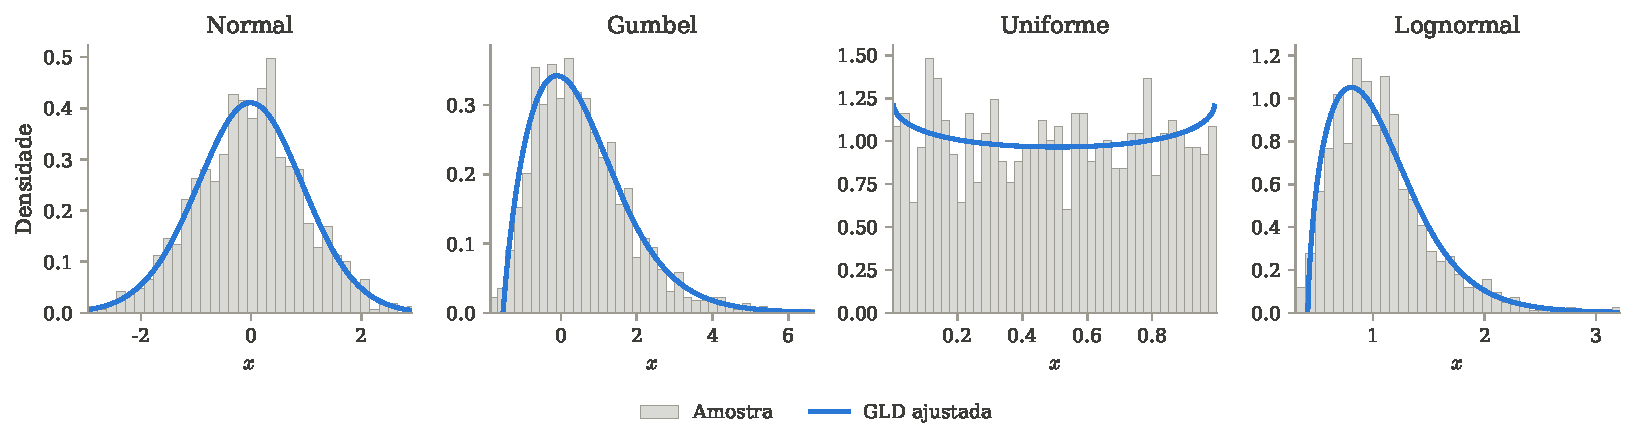
\includegraphics[width=\linewidth]{z_pyglam_fits_pt.pdf}
    \caption{Ajuste da GLD, pelo método dos momentos implementado no PyGLAM, a quatro distribuições-alvo ($N = 1.000$). O histograma corresponde à amostra e a linha contínua à densidade da GLD ajustada.}
    \label{fig:pyglam_fits}
\end{figure}

\begin{table}[htbp]
\centering
\caption{Métricas de qualidade do ajuste da GLD às distribuições-alvo, em média sobre 20 repetições independentes por célula. Erros de quantil normalizados pela amplitude $P_5$--$P_{95}$.}
\label{tab:pyglam_metricas}
\begin{tabular}{lrrrrrrr}
\toprule
\textbf{Distribuição} & \textbf{$N$} & \textbf{KS} & \textbf{$D(q\|p)$} & \textbf{Wasserstein} & \textbf{$P_5$ (\%)} & \textbf{$P_{50}$ (\%)} & \textbf{$P_{95}$ (\%)} \\
\midrule
Normal & 50 & 0,0659 & 0,0488 & 0,0877 & 5,55 & 3,37 & 7,18 \\
 & 200 & 0,0366 & 0,0108 & 0,0512 & 3,59 & 2,04 & 2,27 \\
 & 1.000 & 0,0158 & 0,0021 & 0,0228 & 1,43 & 0,74 & 1,34 \\
 & 5.000 & 0,0059 & 0,0003 & 0,0129 & 0,46 & 0,28 & 0,53 \\
\midrule
Gumbel & 50 & 0,0818 & 0,1047 & 0,1333 & 5,01 & 3,88 & 9,92 \\
 & 200 & 0,0476 & 0,0623 & 0,0947 & 2,46 & 1,57 & 4,94 \\
 & 1.000 & 0,0460 & 0,0941 & 0,0883 & 1,50 & 1,14 & 4,84 \\
 & 5.000 & 0,0436 & 0,0963 & 0,0823 & 1,23 & 0,93 & 3,24 \\
\midrule
Uniforme & 50 & 0,0720 & 0,0341 & 0,0208 & 3,48 & 5,73 & 2,92 \\
 & 200 & 0,0324 & 0,0006 & 0,0099 & 1,16 & 2,41 & 1,39 \\
 & 1.000 & 0,0175 & 0,0026 & 0,0051 & 0,82 & 1,12 & 0,65 \\
 & 5.000 & 0,0066 & 0,0013 & 0,0029 & 0,21 & 0,48 & 0,21 \\
\midrule
Lognormal & 50 & 0,0940 & 0,1238 & 0,0543 & 4,07 & 4,17 & 13,73 \\
 & 200 & 0,0738 & 0,1584 & 0,0423 & 2,74 & 2,56 & 6,36 \\
 & 1.000 & 0,0303 & 0,0481 & 0,0191 & 1,14 & 0,85 & 2,53 \\
 & 5.000 & 0,0149 & 0,0149 & 0,0117 & 0,57 & 0,37 & 1,10 \\
\bottomrule
\end{tabular}
\end{table}

A leitura quantitativa desses resultados é dada pela taxa com que a distância KS decai com o tamanho amostral, obtida por regressão linear em escala logarítmica. O erro de um ajuste por momentos decompõe-se em duas parcelas: uma \textit{amostral}, decorrente da estimação dos quatro primeiros momentos a partir de uma amostra finita, que decai com a taxa teórica $N^{-1/2}$; e outra \textit{estrutural}, decorrente de a família GLD não conter exatamente a distribuição-alvo, que independe de $N$. A inclinação medida discrimina as duas.

Para a Normal e a Uniforme obtiveram-se inclinações de $-0{,}52$ e $-0{,}50$, com $R^2 = 0{,}99$ em ambos os casos --- estatisticamente indistinguíveis da taxa teórica $-1/2$. O erro observado é, portanto, integralmente de natureza amostral, sem parcela estrutural detectável: a GLD representa essas duas distribuições com a precisão que os dados permitirem. Em termos absolutos, em $N = 5.000$ a distância KS cai a 0,0059 e 0,0066, respectivamente, com erros de quantil abaixo de 0,55\% em toda a faixa $P_5$--$P_{95}$. A Lognormal apresenta inclinação de $-0{,}42$, ligeiramente inferior, o que sinaliza uma pequena parcela não amostral, mas ainda converge de forma sustentada, alcançando 1,10\% no $P_{95}$. Esses três casos confirmam a capacidade da GLD de representar simultaneamente distribuições simétricas, assimétricas e de suporte compacto com um único conjunto de quatro parâmetros.

\subsubsection{O limite estrutural da fam\'ilia GLD}

O comportamento da distribuição de Gumbel merece destaque, e a Figura~\ref{fig:pyglam_convergence} o evidencia. Enquanto as demais distribuições decaem com inclinações entre $-0{,}42$ e $-0{,}52$, a curva da Gumbel estabiliza em torno de $\mathrm{KS} \approx 0{,}044$ a partir de $N = 200$: sua inclinação medida é de apenas $-0{,}12$, e o baixo coeficiente de determinação da regressão ($R^2 = 0{,}68$) confirma que o decaimento sequer segue uma lei de potência. Trata-se, portanto, de um patamar \textit{estrutural}, e não amostral: aumentar a amostra não reduz a discrepância porque a família GLD, com os parâmetros de forma ajustados, não representa exatamente a cauda exponencial da Gumbel.

\begin{figure}[htbp]
    \centering
    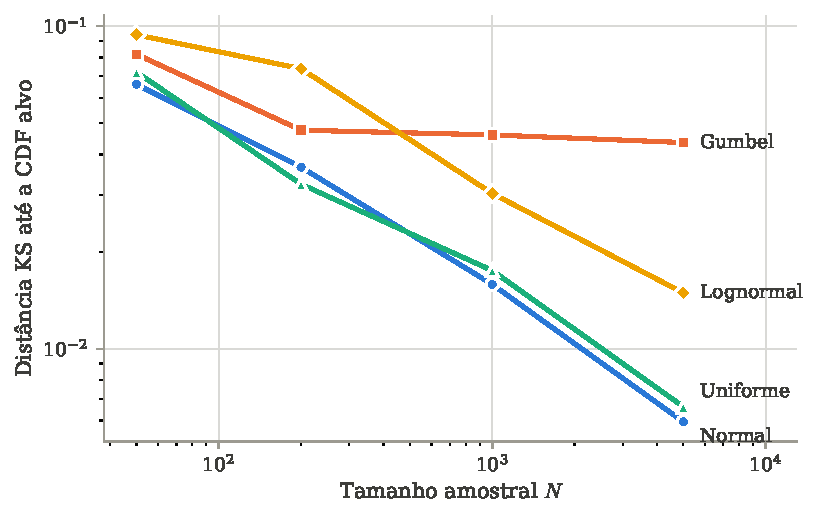
\includegraphics[width=0.62\linewidth]{z_pyglam_convergence_pt.pdf}
    \caption{Convergência da distância de Kolmogorov--Smirnov entre a GLD ajustada e a distribuição-alvo, em função do tamanho amostral. Eixos em escala logarítmica; cada ponto é a média de 20 repetições independentes.}
    \label{fig:pyglam_convergence}
\end{figure}

A mesma leitura explica o comportamento do teste clássico de aderência. Nas 20 repetições, o teste KS de duas amostras não rejeitou a hipótese nula em nenhum caso para a Normal e para a Uniforme, em qualquer tamanho amostral. Para a Gumbel e a Lognormal, contudo, a taxa de rejeição a 5\% cresceu de 0\% em $N = 50$ para 30\% em $N = 5.000$. O aparente paradoxo --- ajustes que melhoram enquanto o teste rejeita mais --- é apenas o ganho de potência do teste: com amostras maiores, ele passa a detectar uma discrepância residual que permanece pequena em magnitude. \textcolor{red}{No Exemplo~\ref{subsec:exemplo1}, a comparação das distribuições é apresentada por métricas de distância e erros de quantis, sem uma decisão de teste de hipótese.}

A origem desse limite é geométrica. Com $\lambda_3, \lambda_4 > 0$, a GLD-FKML tem suporte compacto, de modo que uma distribuição-alvo de suporte ilimitado é necessariamente aproximada por uma de caudas truncadas. Para a Gumbel ajustada em $N = 5.000$, por exemplo, obteve-se $\lambda_3 = 1{,}67$ e $\lambda_4 = 2{,}25$, com suporte $[-1{,}86;\, 34{,}42]$; já a Lognormal produziu $\lambda_4 = -0{,}04$, valor negativo que mantém a cauda direita ilimitada e explica sua convergência mais favorável. Essa constatação é relevante para a interpretação dos resultados de confiabilidade: a aproximação da GLD é excelente no corpo da distribuição e nos quantis usualmente empregados em decisões de manutenção, mas a acurácia na cauda extrema deve ser verificada caso a caso, e não presumida.

% =====================================================================
\subsection{Exemplo 1: verificação em problema de referência}
\label{subsec:exemplo1}

O problema de referência permite avaliar a representação da distribuição de resposta antes da aplicação ao concreto armado. Adota-se uma adaptação do exemplo de \textcite{pires2024}, na qual a margem de segurança depende da resistência $R$, da solicitação $S$ e das incertezas de modelo $Z_1$ e $Z_2$:
\begin{equation}
    g(R,S,t) = k_{\mathrm{fator}}(t)\frac{R}{Z_1} - SZ_2.
    \label{eq:toy_problem_equation}
\end{equation}
A redução da resistência segue a expressão
\begin{equation}
    k_{\mathrm{fator}}(t) =
    \begin{cases}
        1 + (k_{\mathrm{final}}-1)\dfrac{t}{T_f}, & 0 \leq t < T_f, \\[10pt]
        k_{\mathrm{final}},                        & t \geq T_f,
    \end{cases}
    \qquad t\text{ em anos},
    \label{eq:k_factor_linear}
\end{equation}
com $k_{\mathrm{final}} = 0{,}5$ e $T_f = 100$ anos, de modo que a capacidade cai linearmente até metade do valor íntegro ao final do horizonte. Essa magnitude é compatível com uma deterioração severa, ainda que a lei de decaimento permaneça idealizada. A retenção do valor terminal para $t \geq T_f$ é uma salvaguarda: sem ela, a extrapolação linear cruzaria zero em $t = T_f/(1-k_{\mathrm{final}})$ e inverteria o sinal da resistência, produzindo distribuições de resposta degeneradas, sem interpretação física e não representáveis por uma GLD válida. As variáveis de entrada estão descritas na Tabela~\ref{tab:random_variables_parameters}. Esse exemplo representa uma perda idealizada de capacidade e serve à verificação do método. Sua lei de degradação não descreve os mecanismos de carbonatação ou corrosão do concreto armado.

\begin{table}[H]
\centering
\caption{Variáveis do problema de referência.}
\label{tab:random_variables_parameters}
\begin{tabular}{lcccc}
\toprule
Variável & Símbolo & Distribuição & Média & Desvio padrão \\
\midrule
Resistência & $R$ & Normal & 5,00 & 0,80 \\
Solicitação & $S$ & Normal & 2,00 & 0,60 \\
Incerteza de modelo da resistência & $Z_1$ & Lognormal & 1,00 & 0,028 \\
Incerteza de modelo da solicitação & $Z_2$ & Lognormal & 1,00 & 0,096 \\
\bottomrule
\end{tabular}
\end{table}

\subsubsection{Configuração das simulações, representação da GLD e ganho computacional}
\label{subsub:ex1_speedup}

A configuração atual utiliza $2.000$ pontos de projeto para treinamento e $500$ para validação, com $2.500$ realizações de $g$ geradas para cada par $(R,S)$ a partir das variáveis latentes. Os quatro parâmetros da GLD são ajustados às amostras pelo PyGLAM, e os metamodelos PCE são construídos separadamente em cada uma das $5$ idades igualmente espaçadas entre $0$ e $100$ anos. A qualidade desse ajuste, por parâmetro, é discutida na Seção~\ref{subsub:camada_temporal}, junto com o desempenho da camada temporal de aprendizado de máquina.

A distinção entre os dois níveis de amostragem é central para esse ensaio. A variação de $(R,S)$ testa a capacidade de generalização no espaço de entradas, enquanto a repetição de $(Z_1,Z_2)$ para um par fixo determina a distribuição condicional que se deseja emular. As idades $\{0,25,50,75,100\}$ anos cobrem o início, os pontos intermediários e o final da degradação prescrita. Emprega-se uma PCE de grau total máximo cinco, ajustada por mínimos quadrados; sua qualidade é avaliada nos pontos de validação, sem pressupor que o grau escolhido seja ótimo. A lei linear de perda de resistência torna mais simples identificar discrepâncias introduzidas pelo ajuste da GLD e pela representação temporal, antes de introduzir a resposta não linear da carbonatação.

O ganho computacional foi avaliado pela razão entre o tempo do procedimento de referência e o tempo de predição do emulador PCE para o mesmo conjunto de $2.000$ pontos de projeto, em cada uma das cinco idades:
\begin{equation}
    S_{\mathrm{comp}}(t) = \frac{T_{\mathrm{ref}}(t)}{T_{\mathrm{PCE}}(t)}.
    \label{eq:ex1_speedup}
\end{equation}
O tempo $T_{\mathrm{ref}}$ soma a geração das amostras latentes, a avaliação do modelo numérico, a organização dos dados e o ajuste local da GLD. O tempo $T_{\mathrm{PCE}}$ corresponde à predição dos parâmetros para o lote de entradas, com o metamodelo já treinado e carregado. Portanto, a razão mede o ganho na obtenção dos parâmetros da distribuição em relação ao procedimento completo de referência, e não uma comparação com o tempo isolado de avaliação da função $g$.

\begin{table}[H]
\centering
\caption{Tempos por lote de pontos de projeto e ganho computacional nas cinco idades avaliadas.}
\label{tab:computational_time}
\begin{tabular}{rrrr}
\toprule
Tempo (anos) & Referência (s) & Emulador PCE (s) & Ganho (vezes) \\
\midrule
0,00   & 936,209381 & 0,002231 & 419.549 \\
25,00  & 954,884701 & 0,001499 & 637.069 \\
50,00  & 905,878127 & 0,001637 & 553.220 \\
75,00  & 870,398033 & 0,001492 & 583.323 \\
100,00 & 798,989566 & 0,001436 & 556.504 \\
\midrule
Mediana & 905,878127 & 0,001499 & 556.504 \\
\bottomrule
\end{tabular}
\par\smallskip
\begin{minipage}{0.92\linewidth}
\footnotesize A última linha apresenta a mediana de cada coluna, estatística menos sensível ao valor mais baixo registrado em $t=0$. A mediana do ganho é a mediana das cinco razões registradas, calculada antes do arredondamento; não é a razão entre os tempos medianos.
\end{minipage}
\end{table}

O procedimento de referência demandou, na mediana, $905{,}88$~s por idade, enquanto a predição pela PCE levou aproximadamente $1{,}50$~ms. A mediana dos ganhos foi de $5{,}57\times10^5$ vezes, com valores entre $4{,}20\times10^5$ e $6{,}37\times10^5$.

Esses resultados mostram a redução do custo de consulta após a construção da PCE, o que favorece a avaliação repetida de cenários. O treinamento da PCE e o pós-processamento para amostragem, confiabilidade ou RUL não estão incluídos no tempo de predição. Além disso, o registro disponível contém uma cronometragem de predição por idade, sem repetições para estimar sua variabilidade. O ganho obtido caracteriza esse ensaio e não deve ser transferido diretamente para o modelo de durabilidade do concreto.

\subsubsection{Camada temporal de aprendizado de máquina}
\label{subsub:camada_temporal}

A camada temporal utiliza as entradas $(R,S,t)$ para prever os parâmetros $\lambda_1$ e $\lambda_2$ de forma contínua no tempo, dispensando o uso de uma PCE independente para cada instante. Os parâmetros de forma $\lambda_3$ e $\lambda_4$ não são preditos por essa camada, nem pela PCE nas reconstruções distribucionais deste exemplo: como mostra a Tabela~\ref{tab:validation_results}, esses dois parâmetros controlam principalmente as caudas da GLD, variam pouco entre pontos de projeto e ao longo do tempo, e a PCE não os representa com precisão. Adotam-se, portanto, seus valores médios no conjunto de treinamento, $\lambda_3=0{,}142157$ e $\lambda_4=0{,}131525$, nas comparações distribucionais do Exemplo~1. O Exemplo~2 adota seus próprios valores de forma.

\begin{table}[H]
\centering
\caption{Erro quadrático médio (MSE) e coeficiente de determinação $R^2$ dos quatro parâmetros da GLD no conjunto de validação da PCE, por idade.}
\label{tab:validation_results}
\footnotesize
\setlength{\tabcolsep}{4pt}
\begin{tabular}{rrrrrrrrr}
\toprule
 & \multicolumn{4}{c}{MSE} & \multicolumn{4}{c}{$R^2$} \\
\cmidrule(lr){2-5}\cmidrule(lr){6-9}
Tempo (anos) & $\lambda_1$ & $\lambda_2$ & $\lambda_3$ & $\lambda_4$ & $\lambda_1$ & $\lambda_2$ & $\lambda_3$ & $\lambda_4$ \\
\midrule
0,00   & 0,000032 & 0,036096 & 0,000452 & 0,000413 & 0,999969 & 0,979504 & 0,002202      & 0,100693 \\
25,00  & 0,000032 & 0,051272 & 0,000454 & 0,000469 & 0,999965 & 0,976717 & 0,065788      & 0,002610 \\
50,00  & 0,000026 & 0,049197 & 0,000438 & 0,000383 & 0,999967 & 0,984233 & 0,015658      & 0,079338 \\
75,00  & 0,000025 & 0,056486 & 0,000400 & 0,000399 & 0,999962 & 0,986619 & $-0{,}001781$ & 0,060296 \\
100,00 & 0,000022 & 0,063286 & 0,000419 & 0,000420 & 0,999960 & 0,989090 & $-0{,}018763$ & $-0{,}008939$ \\
\bottomrule
\end{tabular}
\end{table}

A predição de $\lambda_1$ tem $R^2$ acima de $0{,}9999$ em todas as idades, com MSE da ordem de $10^{-5}$, cerca de três ordens de grandeza menor que o de $\lambda_2$. Para $\lambda_2$, o $R^2$ fica entre $0{,}977$ e $0{,}989$, com leve melhora nas idades mais avançadas. Já $\lambda_3$ e $\lambda_4$ têm $R^2$ próximo de zero na maior parte da malha temporal, tornando-se negativo para $\lambda_3$ aos $75$ e $100$ anos e para $\lambda_4$ aos $100$ anos: nesses casos, a média dos valores de referência do parâmetro no conjunto de validação produz menor erro quadrático que a predição desse parâmetro pela PCE. Esse comportamento sustenta a escolha de um valor médio fixo para os dois parâmetros de forma, em vez de um metamodelo dedicado a cada um.

A Tabela~\ref{tab:nn_validation} traz as métricas da camada neural global, composta por uma rede para cada parâmetro. Seus alvos são obtidos por 5.000 novas consultas à PCE em cada idade, totalizando 25.000 pares. Assim, as métricas desta tabela medem a reprodução das saídas da PCE pela camada temporal; a comparação com as amostras brutas do simulador é apresentada a seguir.

\begin{table}[H]
\centering
\caption{Erro quadrático médio (MSE) e coeficiente de determinação $R^2$ de $\lambda_1$ e $\lambda_2$ no conjunto de validação da rede neural global.}
\label{tab:nn_validation}
\begin{tabular}{rrrr}
\toprule
MSE $\lambda_1$ & $R^2$ $\lambda_1$ & MSE $\lambda_2$ & $R^2$ $\lambda_2$ \\
\midrule
0,000164 & 0,99989 & 0,00205 & 0,999454 \\
\bottomrule
\end{tabular}
\end{table}

\begin{figure}[H]
    \centering
    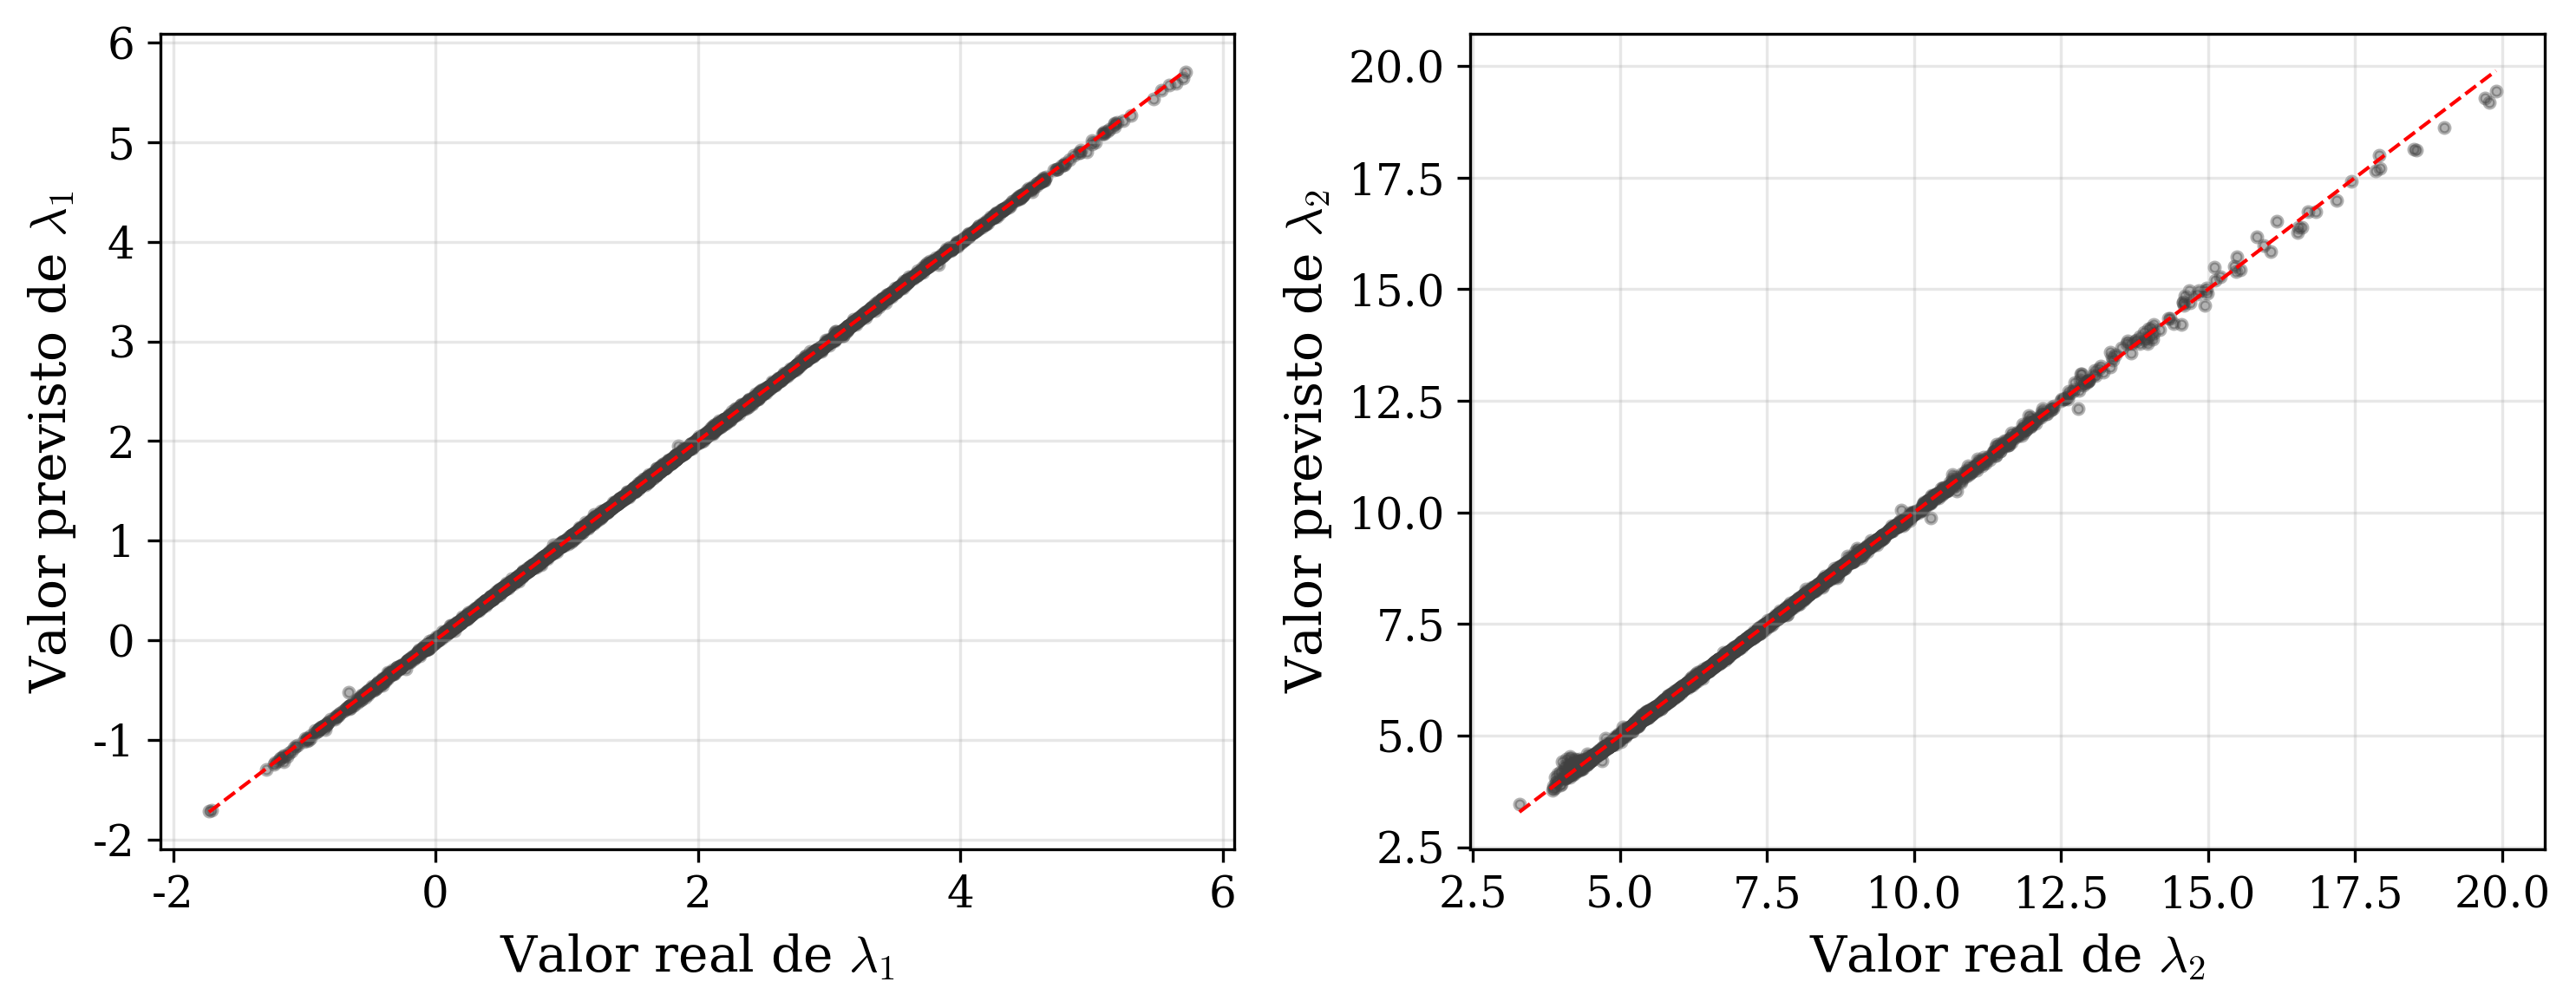
\includegraphics[width=\linewidth]{z_nn_pred_vs_true_pt.png}
    \caption{Valor previsto versus valor real de $\lambda_1$ (esquerda) e $\lambda_2$ (direita) no conjunto de validação da rede neural global. A linha tracejada vermelha marca a identidade.}
    \label{fig:nn_pred_vs_true}
\end{figure}

A camada neural reproduz os alvos gerados pela PCE com $R^2>0{,}9998$ para $\lambda_1$ e $R^2=0{,}999454$ para $\lambda_2$. Como as Tabelas~\ref{tab:validation_results} e~\ref{tab:nn_validation} utilizam referências diferentes, esses valores não demonstram superioridade da rede em relação à PCE na aproximação do simulador físico. A Figura~\ref{fig:nn_pred_vs_true} confirma essa leitura: os pontos se mantêm próximos à identidade em toda a faixa de valores, com dispersão um pouco maior em $\lambda_2$ nos valores mais altos. O resultado é compatível com $\lambda_2$ variar suavemente com $t$: a camada temporal aproveita essa suavidade para interpolar entre os instantes discretos da PCE, em vez de ajustar cada idade isoladamente.

\subsubsection{Propagação de incerteza: PCE versus rede neural}
\label{subsub:propagacao_incerteza}

Esta seção compara diretamente a PCE e a rede neural quanto à propagação de incerteza de $g$, no mesmo ponto de projeto ($R=5{,}394$, $S=2{,}305$, pertencente ao conjunto de treinamento) e nas mesmas duas idades, $t=50$ e $t=100$ anos, com $\lambda_3=0{,}142157$ e $\lambda_4=0{,}131525$ fixados para os dois modelos. A densidade de referência é estimada por KDE sobre as amostras brutas de $g$ desse ponto, e comparada à GLD reconstruída a partir dos parâmetros emulados por cada modelo, pelas métricas da Seção~\ref{subsec:metricas}: divergência KL, estatística KS, distância de Wasserstein, $R^2$ entre densidades e erros relativos de quantil. Por se tratar de um único ponto de projeto, o resultado não generaliza o comportamento dos dois modelos no espaço $(R,S,t)$, mas fornece uma estimativa direta de como cada um se comporta nesse ponto específico.

\begin{figure}[H]
    \centering
    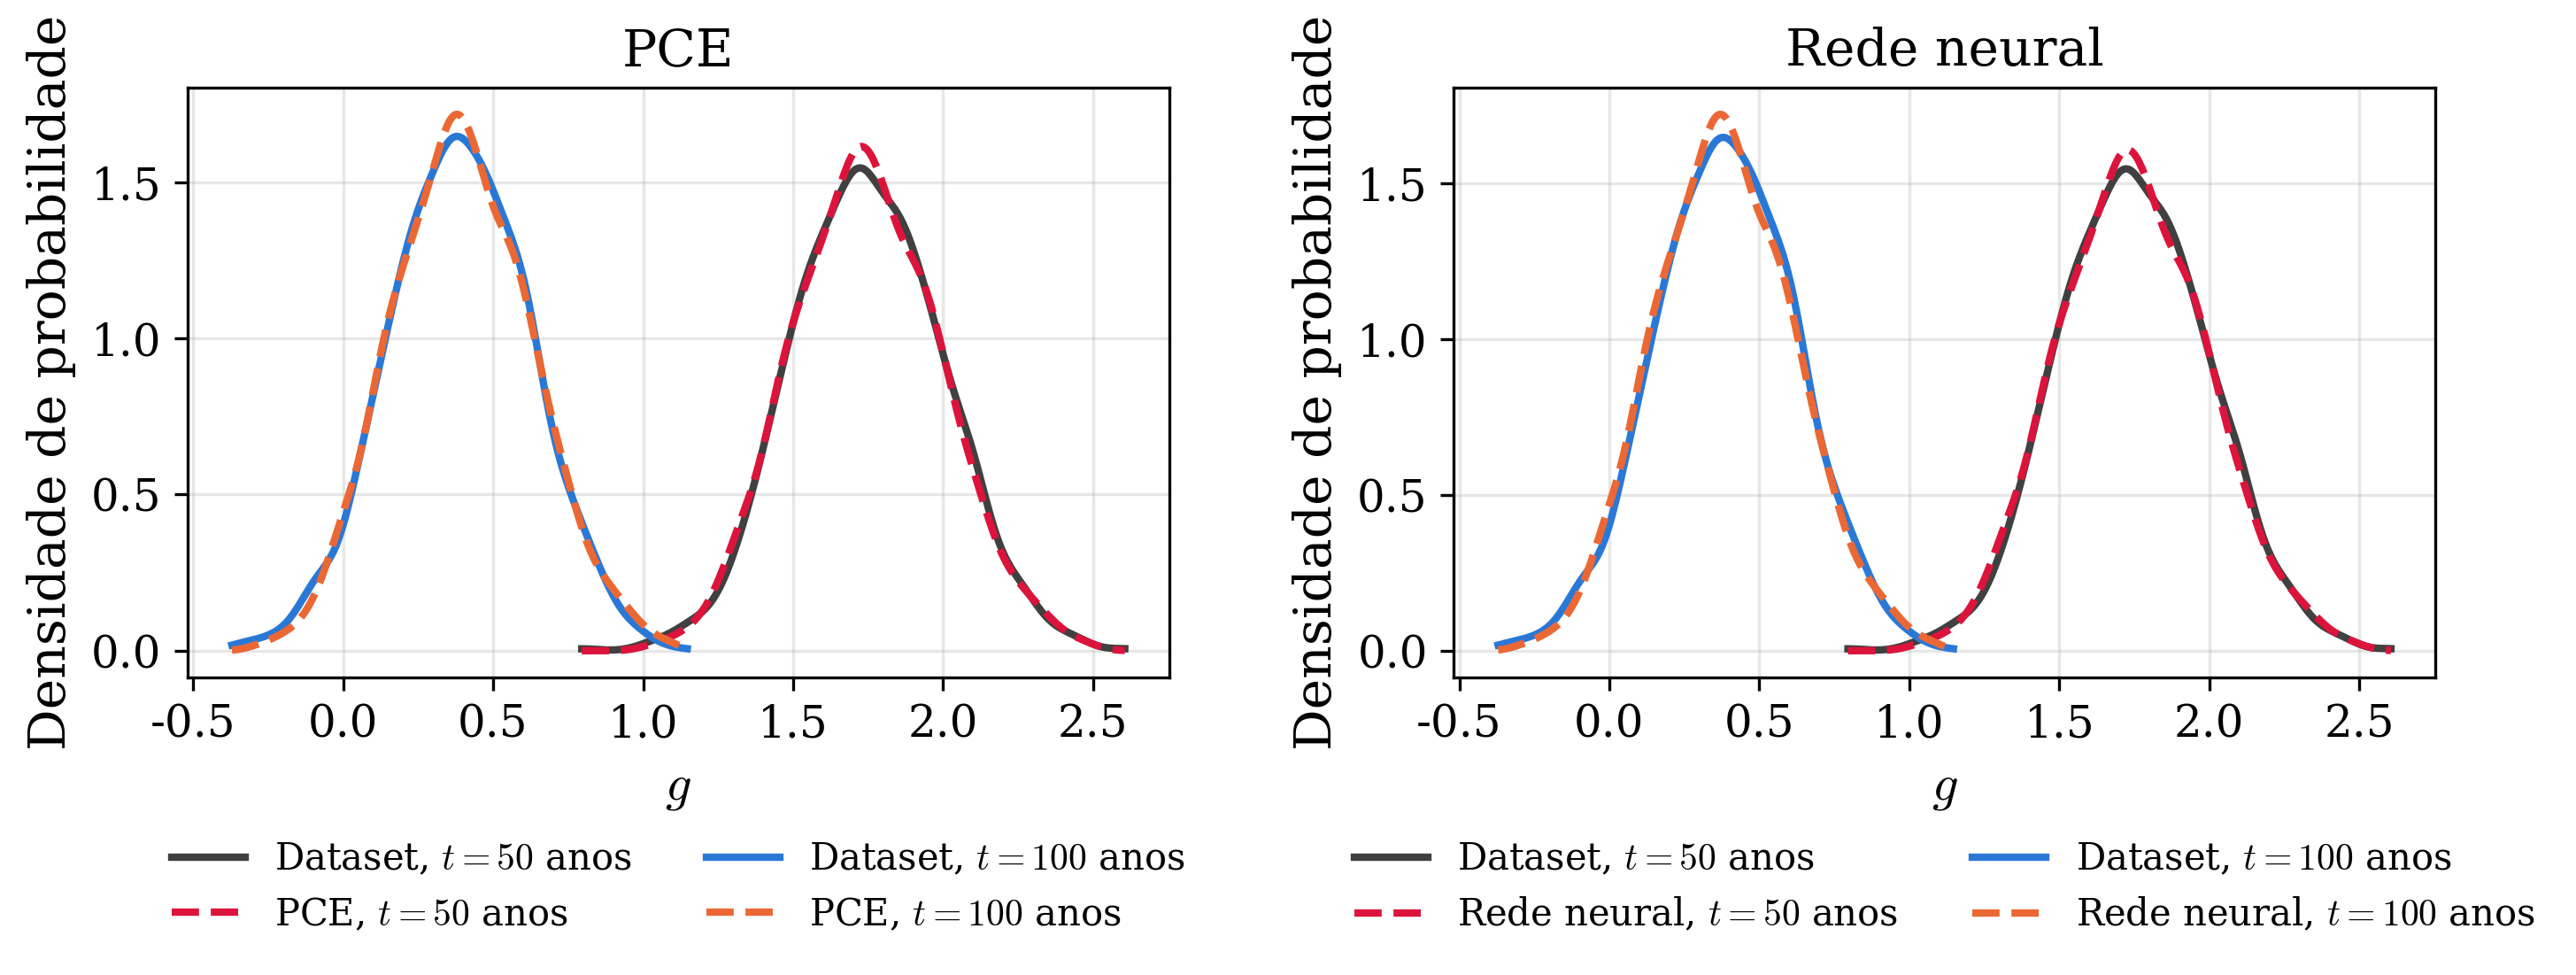
\includegraphics[width=\linewidth]{z_uncertainty_pce_nn_t50_t100_pt.png}
    \caption{Densidades de referência e emuladas para $R=5{,}394$ e $S=2{,}305$, nas idades de $50$ e $100$ anos: PCE (esquerda) e rede neural (direita). A linha cheia representa a KDE das amostras do conjunto de dados e a linha tracejada representa a GLD emulada, com os parâmetros de forma fixados.}
    \label{fig:uncertainty_pce_nn}
\end{figure}

\begin{table}[H]
\centering
\caption{Métricas de propagação de incerteza para a PCE e para a rede neural, no mesmo ponto de projeto, em duas idades.}
\label{tab:uncertainty_propagation}
\begin{tabular}{lrrrr}
\toprule
 & \multicolumn{2}{c}{PCE} & \multicolumn{2}{c}{Rede neural} \\
\cmidrule(lr){2-3}\cmidrule(lr){4-5}
Métrica & $t=50$ & $t=100$ & $t=50$ & $t=100$ \\
\midrule
Divergência KL                 & 0,00374 & 0,00366 & 0,00351 & 0,00318 \\
Estatística KS                 & 0,01840 & 0,01400 & 0,01800 & 0,01960 \\
Distância de Wasserstein       & 0,00540 & 0,00701 & 0,00529 & 0,00740 \\
$R^2$ entre densidades         & 0,99791 & 0,99753 & 0,99801 & 0,99551 \\
Erro relativo em $P_5$ (\%)    & $-0{,}47$ & $+10{,}91$ & $-0{,}61$ & $-46{,}78$ \\
Erro relativo em $P_{50}$ (\%) & $-0{,}16$ & $+0{,}32$  & $-0{,}16$ & $-2{,}05$ \\
Erro relativo em $P_{95}$ (\%) & $+0{,}18$ & $+1{,}11$  & $+0{,}27$ & $-0{,}18$ \\
\bottomrule
\end{tabular}
\end{table}

Aos $50$ anos, PCE e rede neural têm desempenho equivalente e igualmente bom: divergência KL de $0{,}00374$ e $0{,}00351$, $R^2$ acima de $0{,}997$ para ambas, e erros de quantil abaixo de $1\%$ nos três percentis avaliados. As duas curvas praticamente se sobrepõem à KDE de referência na Figura~\ref{fig:uncertainty_pce_nn}.

Aos $100$ anos, a divergência KL favorece discretamente a rede neural, enquanto o $R^2$ entre densidades favorece a PCE ($0{,}00318$ e $0{,}99551$, contra $0{,}00366$ e $0{,}99753$ da PCE). Aqui o $R^2$ da PCE é o maior dos dois, o oposto do que ocorre na divergência KL, o que já sinaliza que essas duas métricas agregadas não contam a mesma história dos quantis. O erro relativo em $P_5$ dispara para os dois modelos, mas de forma assimétrica: $+10{,}91\%$ na PCE contra $-46{,}78\%$ na rede neural. Esse salto não indica necessariamente um colapso do ajuste: aos $100$ anos o percentil $P_5$ do conjunto de referência está próximo de zero (Figura~\ref{fig:uncertainty_pce_nn}, cauda inferior da distribuição à esquerda), de modo que um pequeno desvio absoluto do quantil emulado se traduz em um erro percentual muito maior que nas demais métricas. Ainda assim, a rede neural erra por uma margem consideravelmente maior que a PCE nesse ponto específico, o que é relevante porque a cauda inferior de $g$ é justamente a região que governa a probabilidade de falha.

Em conjunto, os dois ensaios mostram desempenhos globais próximos, com diferenças de ordenação entre as métricas e maior erro relativo da rede neural na cauda inferior aos 100 anos. Um único ponto de projeto não permite afirmar se isso é uma característica sistemática do modelo global ou uma particularidade deste ponto e desta idade. \falta{Repetir esta comparação em outros pontos de projeto e idades para verificar se a maior sensibilidade da rede neural na cauda inferior em $t=100$ é sistemática.}

\subsubsection{Vida útil remanescente}

Para este exemplo, adota-se um limiar de intervenção em $g=0{,}7$, definido apenas para fins de ilustração do método, sem correspondência com um critério normativo específico. O fim da vida útil é tomado como o primeiro instante em que $g$ cruza esse limiar, e não necessariamente $g=0$: na prática, uma intervenção de manutenção é programada enquanto ainda resta margem de segurança, não apenas quando o estado limite já foi atingido.

\begin{figure}[H]
    \centering
    \begin{subfigure}[b]{0.48\textwidth}
        \centering
        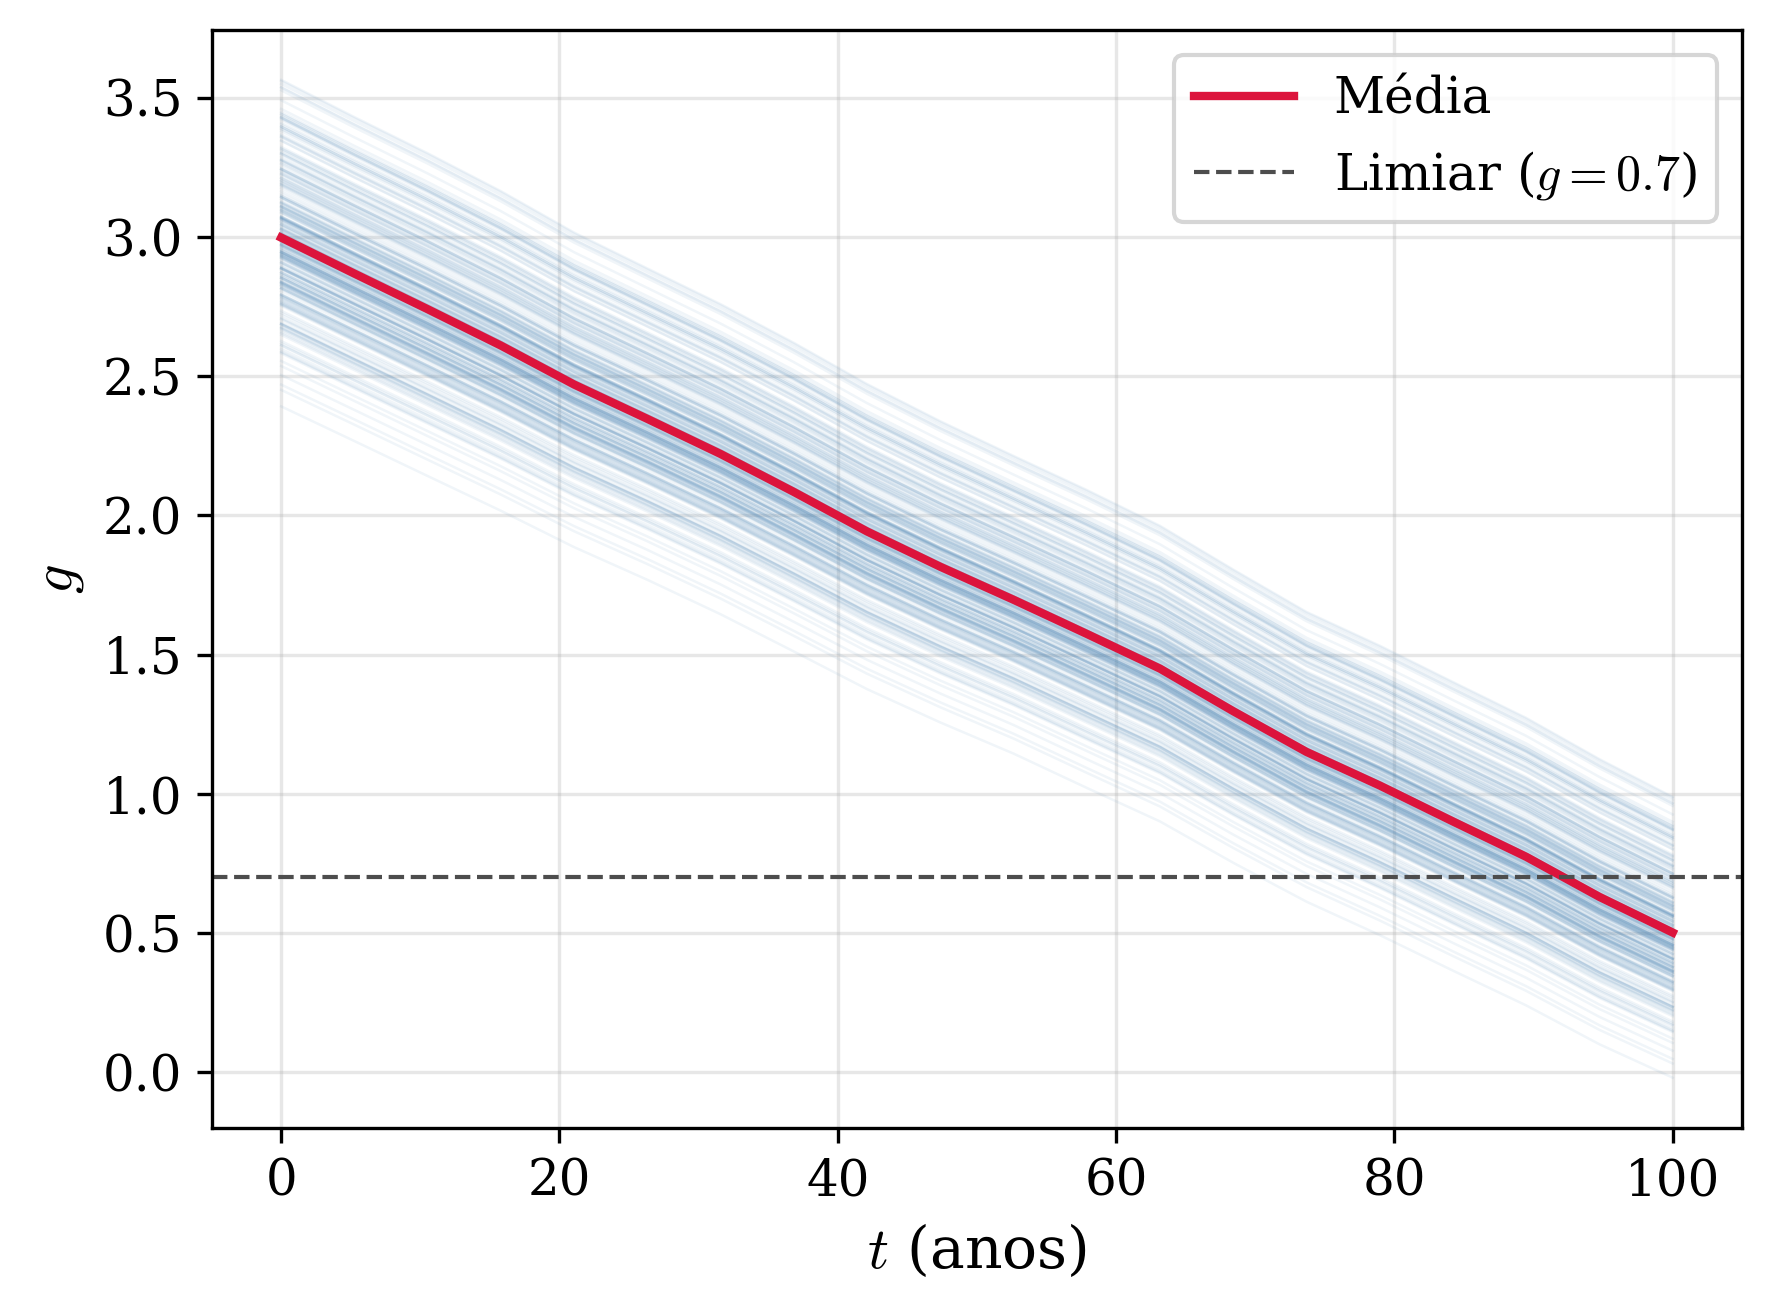
\includegraphics[width=\linewidth]{z_rul_spaghetti_R5_S2_pt.png}
        \caption{Trajetórias de $g(t)$.}
        \label{fig:rul_spaghetti}
    \end{subfigure}
    \hfill
    \begin{subfigure}[b]{0.48\textwidth}
        \centering
        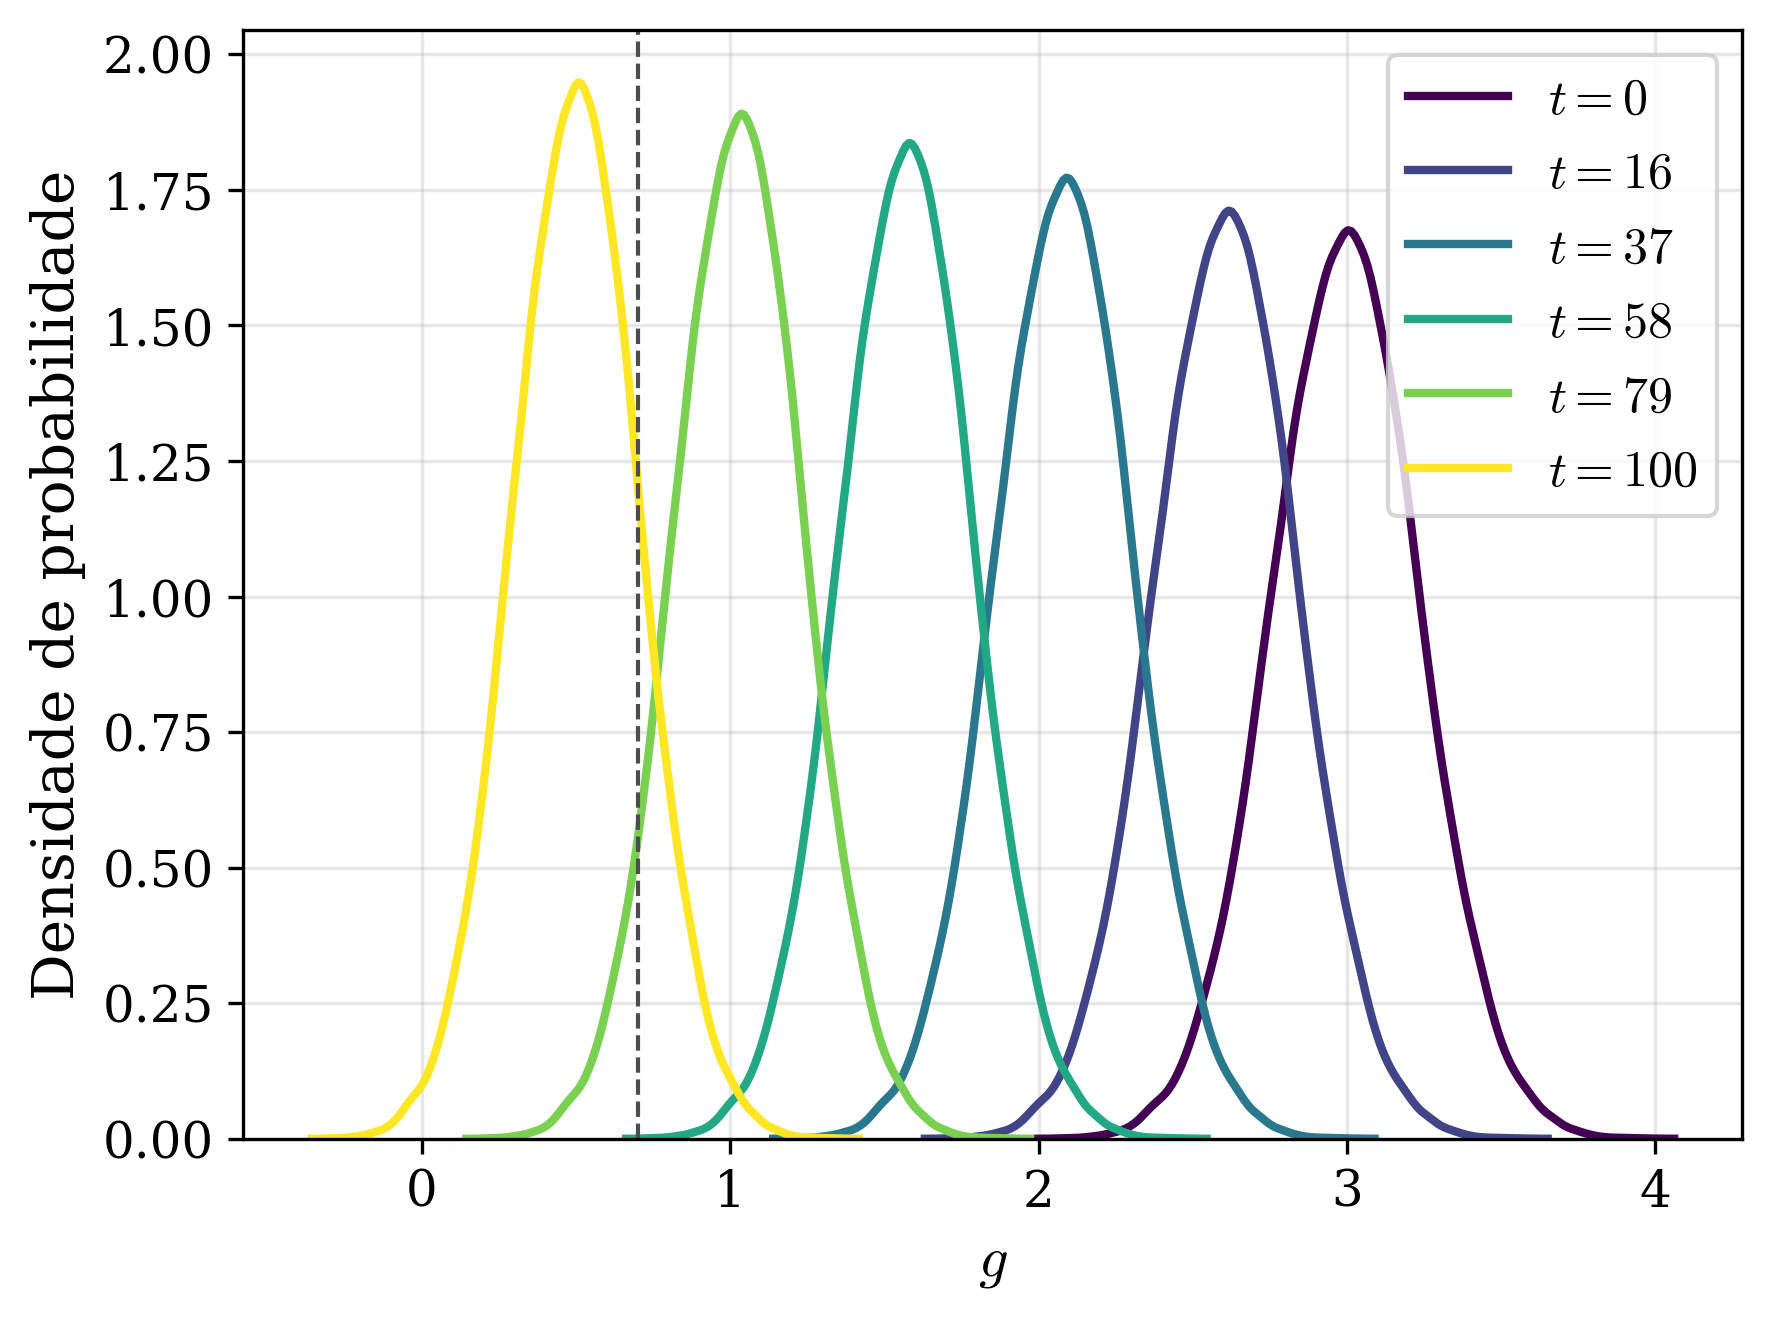
\includegraphics[width=\linewidth]{2500_rul_samples_R5_S2_benchmark_g_pdfs_pt.png}
        \caption{Densidade de $g$ em seis idades.}
        \label{fig:rul_g_pdfs}
    \end{subfigure}
    \caption{Comportamento de $g(t)$ para $R=5{,}0$ e $S=2{,}0$ (valores médios das variáveis de entrada): (a) $300$ das $50.000$ trajetórias simuladas, com a média (vermelho); (b) densidade de $g$ em seis idades entre $0$ e $100$ anos. O limiar de intervenção $g=0{,}7$ é indicado em ambos os painéis (tracejado).}
    \label{fig:rul_trajetorias}
\end{figure}

Cada trajetória do painel (a) é comonotônica: um único nível de quantil $u$ é sorteado por trajetória e mantido fixo ao longo do tempo, de modo que $g_i(t) = Q\!\left(u_i; \hat{\boldsymbol{\lambda}}(t)\right)$, o que preserva a ordenação das realizações entre as idades. A monotonicidade no tempo depende da evolução dos quantis emulados e deve ser verificada separadamente. Amostrar cada instante de forma independente produziria, em vez disso, trajetórias que oscilam livremente. A dispersão entre trajetórias cresce com o tempo, conforme a evolução da dispersão condicional representada pelos parâmetros da GLD, e a média cruza o limiar por volta de $t=91$ anos. O painel (b) mostra a mesma degradação sob outro ângulo: a densidade de $g$ se desloca gradualmente para a esquerda, e por $t=100$ anos seu corpo já ultrapassou o limiar.

\begin{figure}[H]
    \centering
    \begin{subfigure}[b]{0.48\textwidth}
        \centering
        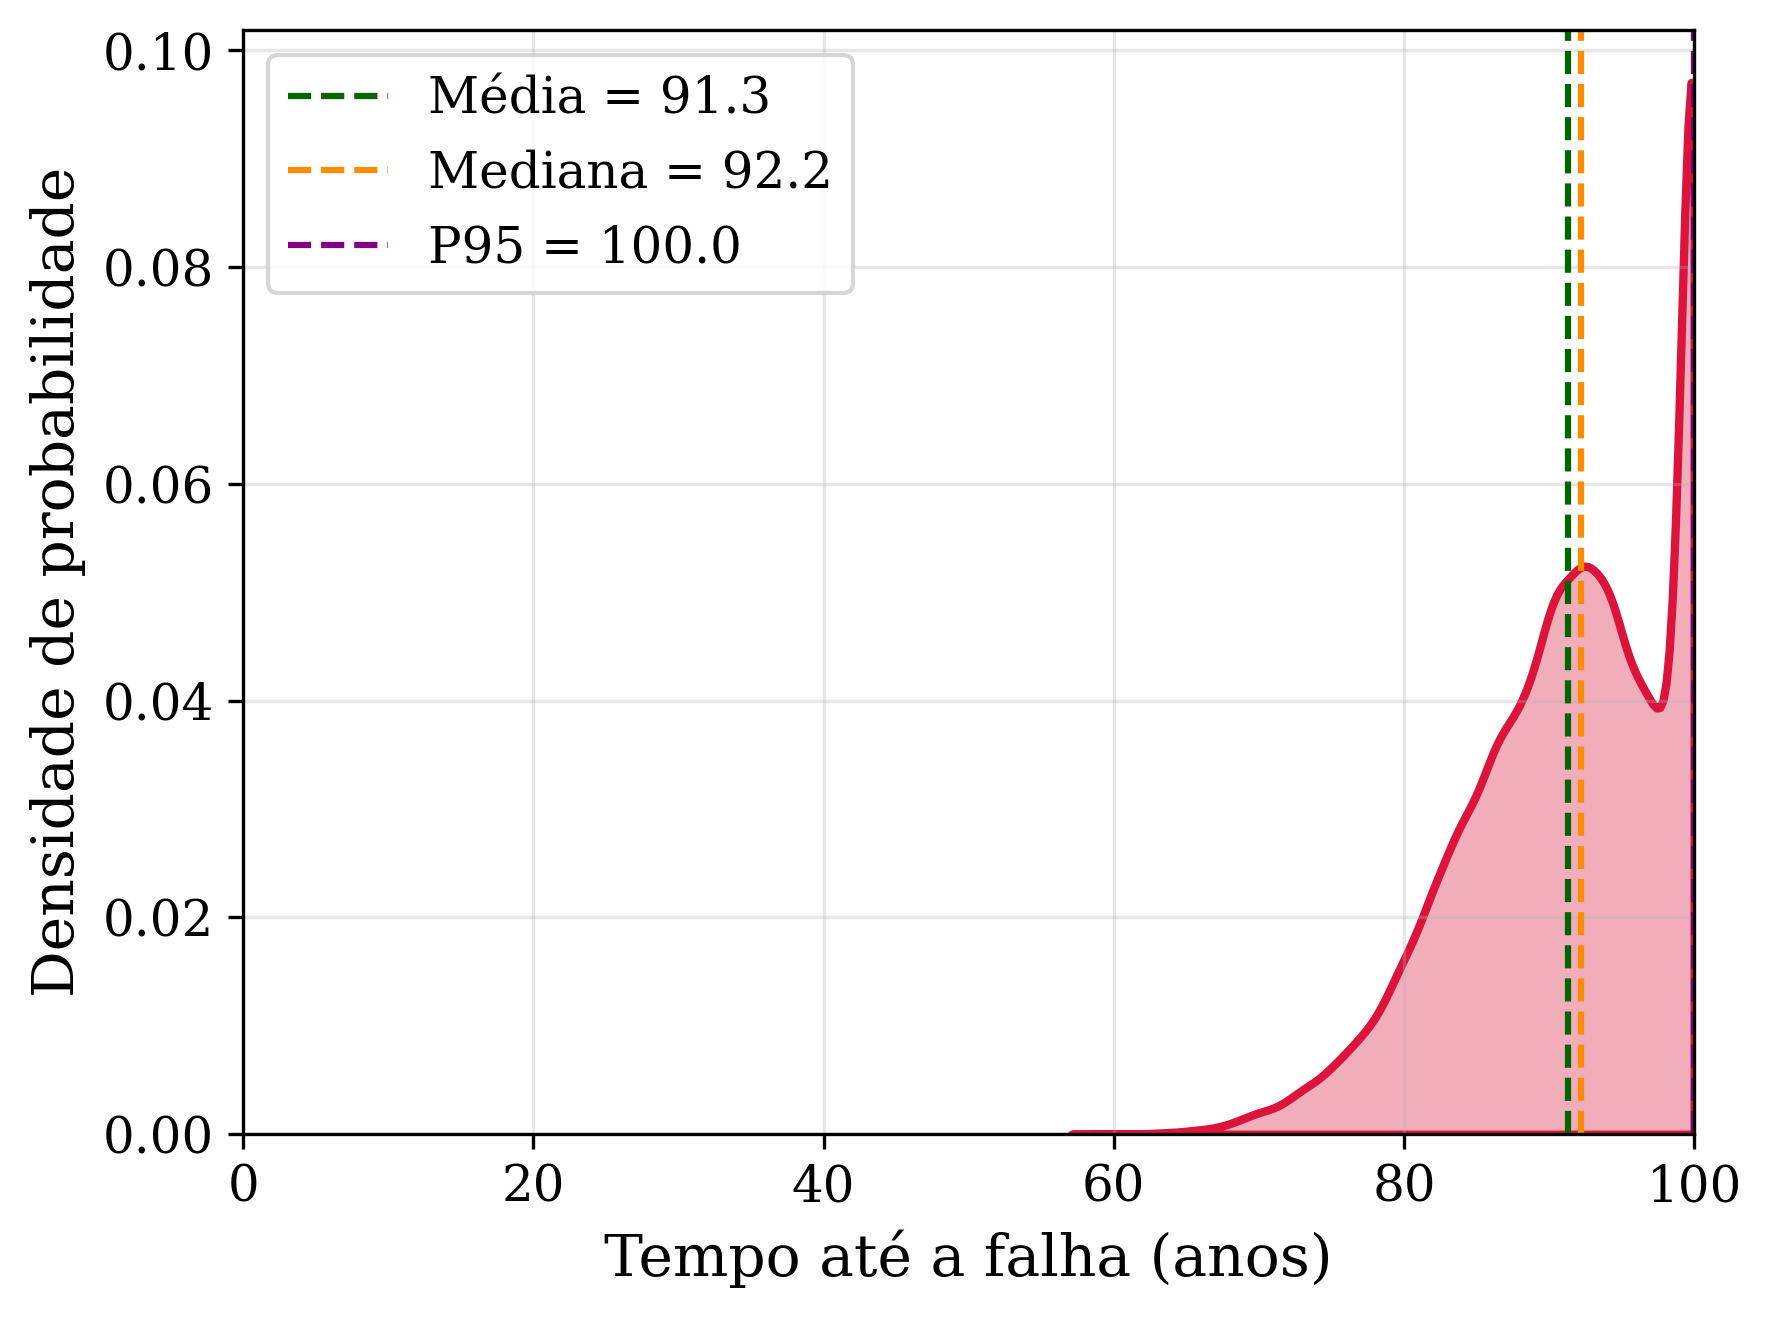
\includegraphics[width=\linewidth]{2500_rul_samples_R5_S2_benchmark_rul_pdf_pt.png}
        \caption{Tempo até o cruzamento, a partir de $t=0$.}
        \label{fig:rul_pdf}
    \end{subfigure}
    \hfill
    \begin{subfigure}[b]{0.48\textwidth}
        \centering
        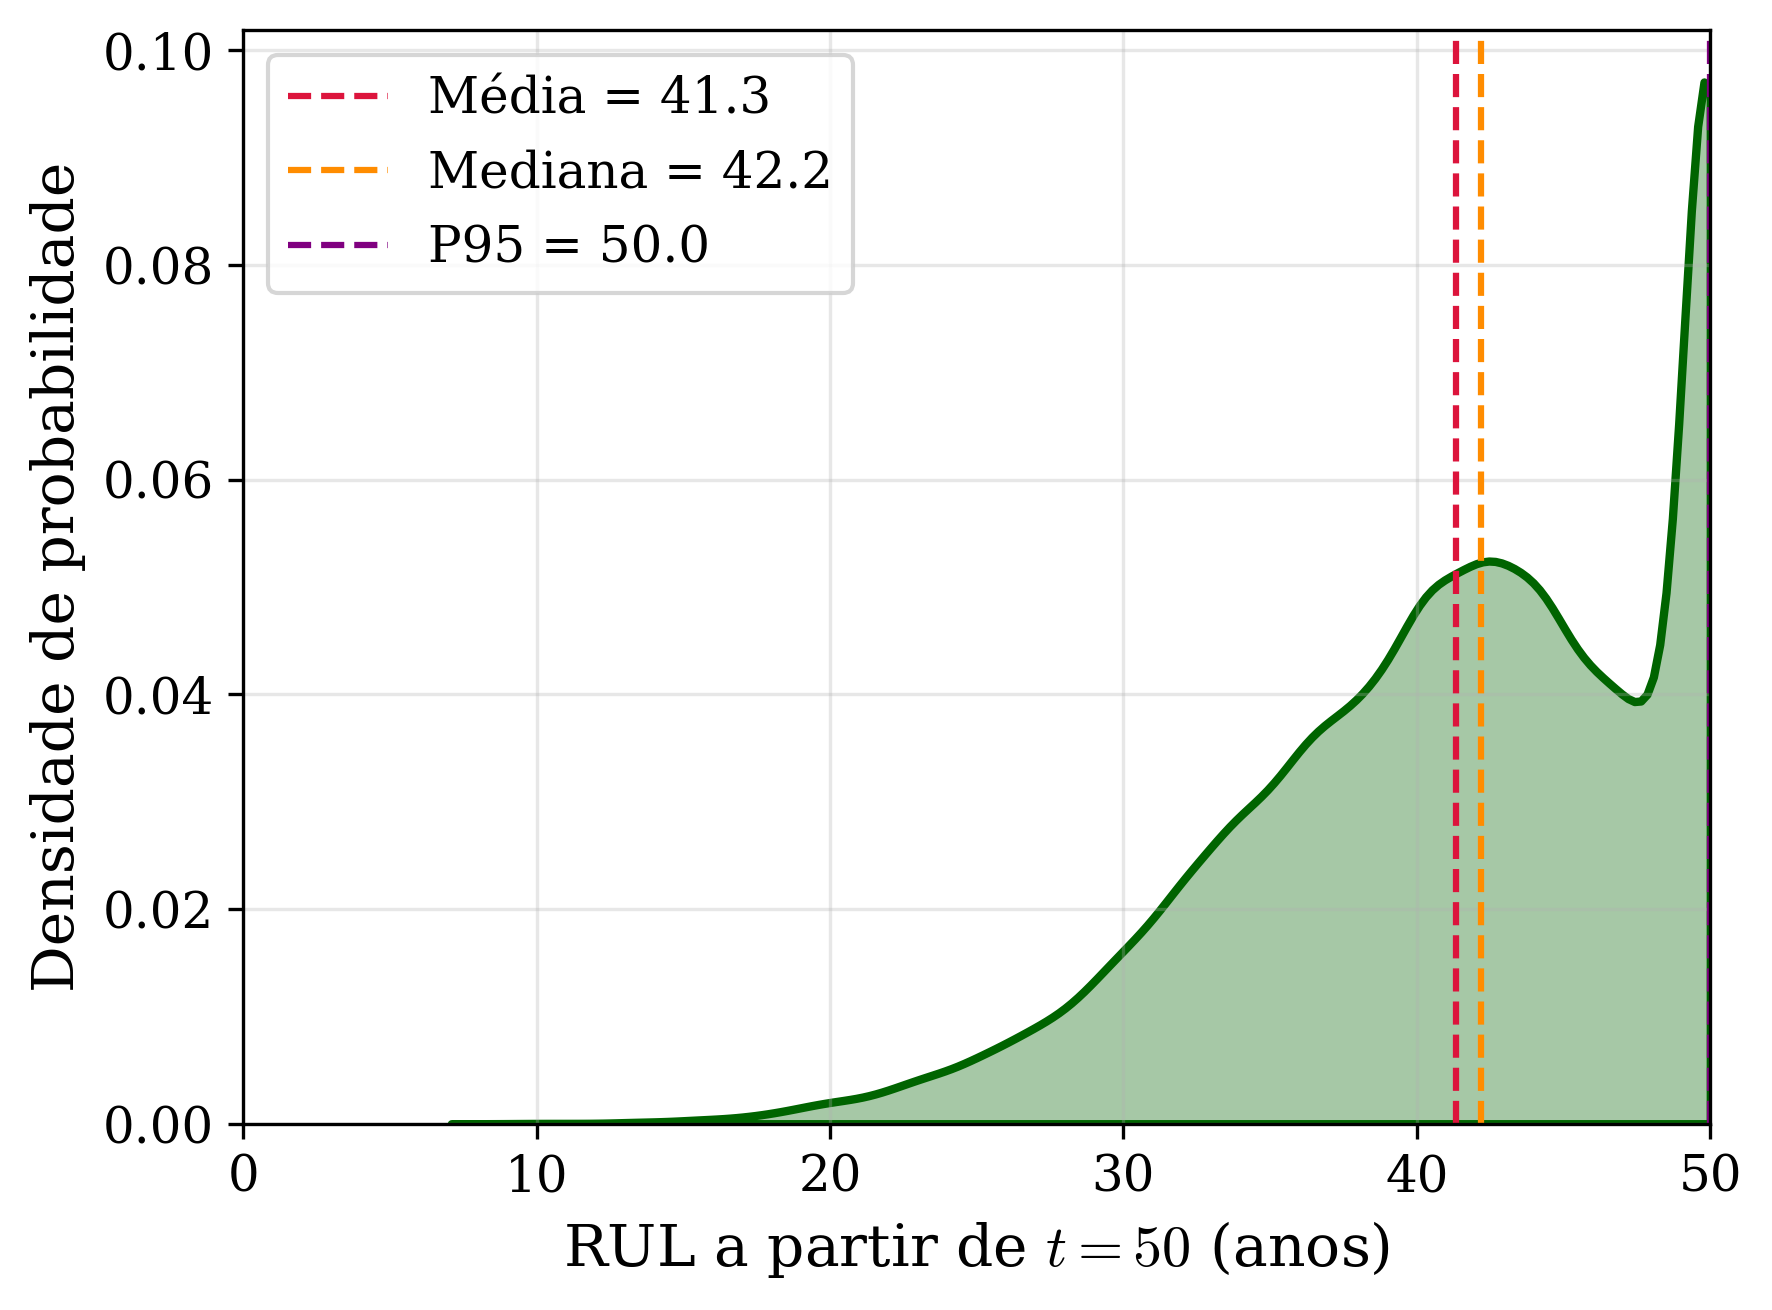
\includegraphics[width=\linewidth]{2500_rul_samples_R5_S2_benchmark_conditional_rul_t50_pt.png}
        \caption{RUL condicionada à sobrevivência em $t=50$ anos.}
        \label{fig:rul_conditional}
    \end{subfigure}
    \caption{Distribuição do tempo até o cruzamento do limiar $g=0{,}7$, para $R=5{,}0$ e $S=2{,}0$: (a) a partir de $t=0$; (b) vida útil remanescente condicionada à sobrevivência em $t=50$ anos, $\mathrm{RUL}=T-t_{\mathrm{insp}}$. Ambas as densidades são truncadas no maior valor alcançável dentro do horizonte simulado de $100$ anos.}
    \label{fig:rul_distribuicoes}
\end{figure}

Os tempos armazenados, limitados ao horizonte de 100 anos, apresentam média restrita de $91{,}32$ anos, mediana de $92{,}18$ anos, desvio padrão de $7{,}13$ anos e $P_5=78{,}19$ anos, com $16{,}4\%$ das trajetórias censuradas em $t=100$ anos. O pico estreito junto a esse limite corresponde a essa censura, não a um comportamento intrínseco da distribuição. Como nenhuma trajetória cruza o limiar antes de $t=50$ anos (valor obtido por interpolação linear entre os instantes simulados, que não incluem $t=50$ diretamente), todas as $50.000$ sobrevivem até esse instante, e a RUL condicional do painel (b) é a mesma distribuição do painel (a), apenas deslocada em $50$ anos: média restrita de $41{,}32$ anos e mediana de $42{,}18$ anos. O percentil empírico $P_{95}=50{,}00$ anos recai no limite do horizonte: a simulação não determina o percentil 95 da RUL completa.

% =====================================================================
\subsection{Exemplo 2: distribuição da margem de durabilidade e vida remanescente sob carbonatação}
\label{subsec:exemplo2}

O segundo exemplo investiga se o emulador consegue representar a evolução da distribuição de $g=c-y(t)$ quando a degradação decorre do modelo de carbonatação da Seção~\ref{subsec:modelo_possan}. O caso corresponde a um elemento de concreto armado idealizado, com início da exposição em 1980, cimento CP~II~F, ambiente externo protegido da chuva e concentração atmosférica de CO$_2$ segundo SSP2-4.5. A análise compreende as idades de zero a 100 anos, correspondentes a 1980--2080. Essas definições caracterizam um estudo numérico; não se atribuem os parâmetros a uma estrutura inspecionada.

\subsubsection{Escolha das entradas e do ponto de análise}

O domínio de construção do emulador está apresentado na Tabela~\ref{tab:viga_va}. As três entradas são amostradas de distribuições uniformes independentes. Aqui, essas distribuições definem a cobertura do espaço de estudo: cada ponto representa uma combinação nominal de concreto, ambiente e cobrimento. A dispersão da resposta para um elemento com entradas fixadas é introduzida separadamente pelas variáveis latentes da Seção~\ref{subsec:parametrizacao}.

\begin{table}[htbp]
\centering
\caption{Domínio das entradas e ponto fixado para a análise de vida remanescente do Exemplo~2. A umidade é apresentada em porcentagem e convertida em fração na equação de carbonatação.}
\label{tab:viga_va}
\begin{tabular}{lccc}
\toprule
Entrada & Símbolo & Domínio de amostragem & Ponto fixado \\
\midrule
Resistência à compressão & $f_c$ & $\mathcal{U}(20,50)$ MPa & 25 MPa \\
Umidade relativa & $UR$ & $\mathcal{U}(20,80)$\% & 55\% \\
Cobrimento nominal & $c_{\mathrm{nom}}$ & $\mathcal{U}(15,60)$ mm & 25 mm \\
\bottomrule
\end{tabular}
\end{table}

As entradas exercem papéis distintos na função de estado limite. O cobrimento desloca diretamente a margem de segurança, pois representa a distância que a frente carbonatada precisa percorrer para alcançar a armadura. A resistência à compressão modifica a profundidade prevista pelo modelo, e a umidade relativa atua de forma não monotônica: o termo quadrático da Equação~\eqref{eq:y} atinge seu máximo em $UR=58\%$. Assim, a faixa de umidade abrange ambos os lados desse máximo e exige que o emulador represente respostas diferentes para ambientes mais secos e mais úmidos. Esses intervalos constituem o domínio numérico escolhido; a sua adoção não equivale à validação experimental do modelo em toda a faixa, conforme discutido na Seção~\ref{subsec:modelo_possan}.

Para a análise temporal detalhada, fixa-se $(f_c,UR,c_{\mathrm{nom}})=(25\,\mathrm{MPa},55\%,25\,\mathrm{mm})$. A resistência e o cobrimento situam-se na parte inferior dos respectivos intervalos, enquanto a umidade está próxima daquela que maximiza a profundidade no modelo. Essa combinação permite examinar uma condição favorável ao avanço da carbonatação e acompanhar a aproximação de $g$ aos limiares de interesse. A ocorrência e o instante de cruzamento permanecem resultados da análise probabilística. Os valores escolhidos não constituem uma especificação normativa de projeto.

A escolha de 1980 estabelece uma origem temporal para avaliar um elemento que envelhece sob uma trajetória ambiental variável. O cenário SSP2-4.5 é mantido fixo para que a análise se concentre na variabilidade das entradas e na aproximação pelo emulador; não lhe é atribuída probabilidade de ocorrência. O horizonte de 100 anos permanece dentro da série ambiental disponível. Na parametrização do cimento, adota-se $ad=0\%$, representando a hipótese de ausência de adição pozolânica suplementar, conforme a Seção~\ref{subsec:parametrizacao}.

\subsubsection{Variabilidade condicional e construção do conjunto de dados}

Para cada combinação nominal são geradas $2.500$ réplicas independentes dos multiplicadores de resistência, umidade e cobrimento. Os multiplicadores da resistência e do cobrimento são lognormais com média unitária e coeficiente de variação de $15\%$; o da umidade é obtido de uma Normal de média unitária e desvio padrão $0{,}15$, truncada para manter a umidade efetiva entre zero e $100\%$. As distribuições positivas evitam valores negativos de resistência e cobrimento. A truncagem da umidade respeita seu intervalo físico sem acumular artificialmente observações exatamente nos limites. Como a truncagem altera os momentos, o coeficiente de variação efetivo da umidade não é exatamente $15\%$ em todos os pontos de projeto.

O valor comum de $15\%$ define a intensidade de dispersão adotada no experimento. Ele permite estudar a propagação de uma variabilidade não desprezível, mas não é tratado como uma calibração conjunta das três grandezas para uma obra real. A influência dessa hipótese sobre a vida remanescente deve ser considerada na interpretação dos resultados; sua eventual aplicação a um ativo específico requer caracterização própria dos materiais, do cobrimento e da exposição.

São amostrados $2.000$ pontos de treinamento e $500$ pontos de validação, mantidos nas cinco idades $\{0,25,50,75,100\}$ anos. A reutilização das mesmas entradas permite acompanhar a evolução da distribuição em cada ponto. As réplicas latentes são geradas novamente em cada idade; portanto, o conjunto de treinamento caracteriza distribuições condicionais e não fornece, por si só, trajetórias individuais acompanhadas ao longo do tempo. O planejamento corresponde a $25$ milhões de respostas escalares de $g$ para treinamento e $6{,}25$ milhões para validação, totalizando $12.500$ ajustes locais de GLD pelo método dos momentos, com 15 inicializações do procedimento de ajuste.

Convém distinguir a malha do simulador físico da malha de treinamento. O simulador avalia a expressão de carbonatação em uma malha auxiliar de dez anos, aplica o máximo acumulado da profundidade e interpola linearmente para obter a resposta na idade consultada. As cinco idades de treinamento selecionam as distribuições a serem aproximadas pela PCE. Essa organização reduz o número de ajustes distribucionais ao longo do tempo, mas introduz uma discretização que precisa ser considerada na avaliação da precisão temporal.

\subsubsection{PCE e camada temporal}

Em cada idade ajusta-se uma PCE de grau total máximo três por mínimos quadrados aos quatro parâmetros locais da GLD. Para três entradas, essa escolha resulta em 20 termos por parâmetro, incluindo a constante, estimados com $2.000$ pontos de treinamento. A relação entre o número de pontos e o número de termos produz um ajuste sobredeterminado. O grau três constitui a configuração inicial do estudo; sua suficiência deve ser avaliada pelos erros nos pontos de validação, sobretudo em regiões de maior curvatura da resposta em função da umidade.

A camada temporal recebe $(f_c,UR,c_{\mathrm{nom}},t)$ e é treinada a partir de $5.000$ novas consultas a cada PCE, totalizando até $25.000$ pares de entrada e saída. Esses alvos são predições das PCEs. A geração dessa base mais densa permite treinar a rede sem repetir as simulações físicas e os ajustes locais da GLD. Antes do treinamento são excluídas as linhas com $\lambda_2\leq0$ e as linhas com alvos ausentes. A quantidade descartada deve acompanhar as métricas, pois a exclusão pode reduzir a cobertura do domínio.

São utilizadas duas redes do tipo perceptron multicamadas, uma para $\lambda_1$ e outra para $\lambda_2$, cada qual com duas camadas ocultas de 64 neurônios. As entradas são padronizadas a partir do subconjunto de treinamento. Adotam-se uma partição aleatória de $80\%$ para treinamento e $20\%$ para validação, no máximo 500 iterações e parada antecipada com tolerância de 15 iterações sem melhoria; a semente da partição e das redes é 42. A mesma arquitetura do problema de referência permite comparar a aplicação do procedimento aos dois exemplos sem introduzir uma seleção adicional de regressores.

Na reconstrução das distribuições adotam-se $\lambda_3=0{,}198312$ e $\lambda_4=0{,}130039$, médias dos ajustes locais no conjunto de treinamento na execução com $ad=0\%$ e variabilidade latente de $15\%$. Das $25.000$ linhas geradas para a base temporal, nenhuma foi descartada pelo critério $\lambda_2\leq0$ ou por alvo ausente, de modo que a rede foi treinada sobre a totalidade das consultas às PCEs, com $20.000$ linhas para treinamento e $5.000$ para validação.

A Tabela~\ref{tab:validation_results_ex2} apresenta o MSE e o $R^2$ dos quatro parâmetros da PCE nos $500$ pontos de validação, por idade. Como no Exemplo~1, $\lambda_1$ é o parâmetro mais bem representado, com $R^2$ acima de $0{,}997$ em todas as idades; $\lambda_2$ mantém $R^2$ entre $0{,}884$ e $0{,}983$. Os parâmetros de forma $\lambda_3$ e $\lambda_4$ têm $R^2$ próximo de zero ou negativo em quase todas as idades --- chegando a $-1{,}28$ para $\lambda_4$ aos 25 anos ---, o que reforça a opção por fixá-los em seus valores médios em vez de emulá-los pela PCE.

\begin{table}[H]
\centering
\caption{Erro quadrático médio (MSE) e coeficiente de determinação $R^2$ dos quatro parâmetros da GLD no conjunto de validação da PCE, por idade, no Exemplo~2.}
\label{tab:validation_results_ex2}
\footnotesize
\setlength{\tabcolsep}{4pt}
\begin{tabular}{rrrrrrrrr}
\toprule
 & \multicolumn{4}{c}{MSE} & \multicolumn{4}{c}{$R^2$} \\
\cmidrule(lr){2-5}\cmidrule(lr){6-9}
Tempo (anos) & $\lambda_1$ & $\lambda_2$ & $\lambda_3$ & $\lambda_4$ & $\lambda_1$ & $\lambda_2$ & $\lambda_3$ & $\lambda_4$ \\
\midrule
0,00   & 0,244947 & 0,000388 & 0,201466 & 0,445823 & 0,998568 & 0,976155 & 0,005321      & 0,005749 \\
25,00  & 0,131674 & 0,000143 & 0,001815 & 0,002885 & 0,999299 & 0,982971 & 0,457648      & $-1{,}280777$ \\
50,00  & 0,327814 & 0,000195 & 0,125826 & 0,081558 & 0,998430 & 0,970964 & $-0{,}078117$ & $-0{,}039379$ \\
75,00  & 0,458894 & 0,000710 & 0,437726 & 0,370454 & 0,998003 & 0,884269 & $-0{,}039640$ & $-0{,}011561$ \\
100,00 & 0,623390 & 0,000295 & 0,303531 & 0,148885 & 0,997524 & 0,946618 & $-0{,}044526$ & $-0{,}000625$ \\
\bottomrule
\end{tabular}
\end{table}

A Tabela~\ref{tab:nn_validation_ex2} traz as métricas da camada neural global na partição de validação da base gerada pelas PCEs. A escala de $\lambda_1$ neste exemplo (profundidade em milímetros, tipicamente entre 0 e 50~mm) é maior que a do Exemplo~1, o que explica o MSE absoluto mais alto sem indicar pior ajuste relativo: o $R^2$ de $0{,}999542$ para $\lambda_1$ e $0{,}999354$ para $\lambda_2$ é comparável ao obtido no problema de referência.

\begin{table}[H]
\centering
\caption{Erro quadrático médio (MSE) e coeficiente de determinação $R^2$ de $\lambda_1$ e $\lambda_2$ no conjunto de validação da rede neural global do Exemplo~2.}
\label{tab:nn_validation_ex2}
\begin{tabular}{rrrr}
\toprule
MSE $\lambda_1$ & $R^2$ $\lambda_1$ & MSE $\lambda_2$ & $R^2$ $\lambda_2$ \\
\midrule
0,110126 & 0,999542 & 0,000006 & 0,999354 \\
\bottomrule
\end{tabular}
\end{table}

\begin{figure}[H]
    \centering
    \begin{subfigure}[b]{0.48\textwidth}
        \centering
        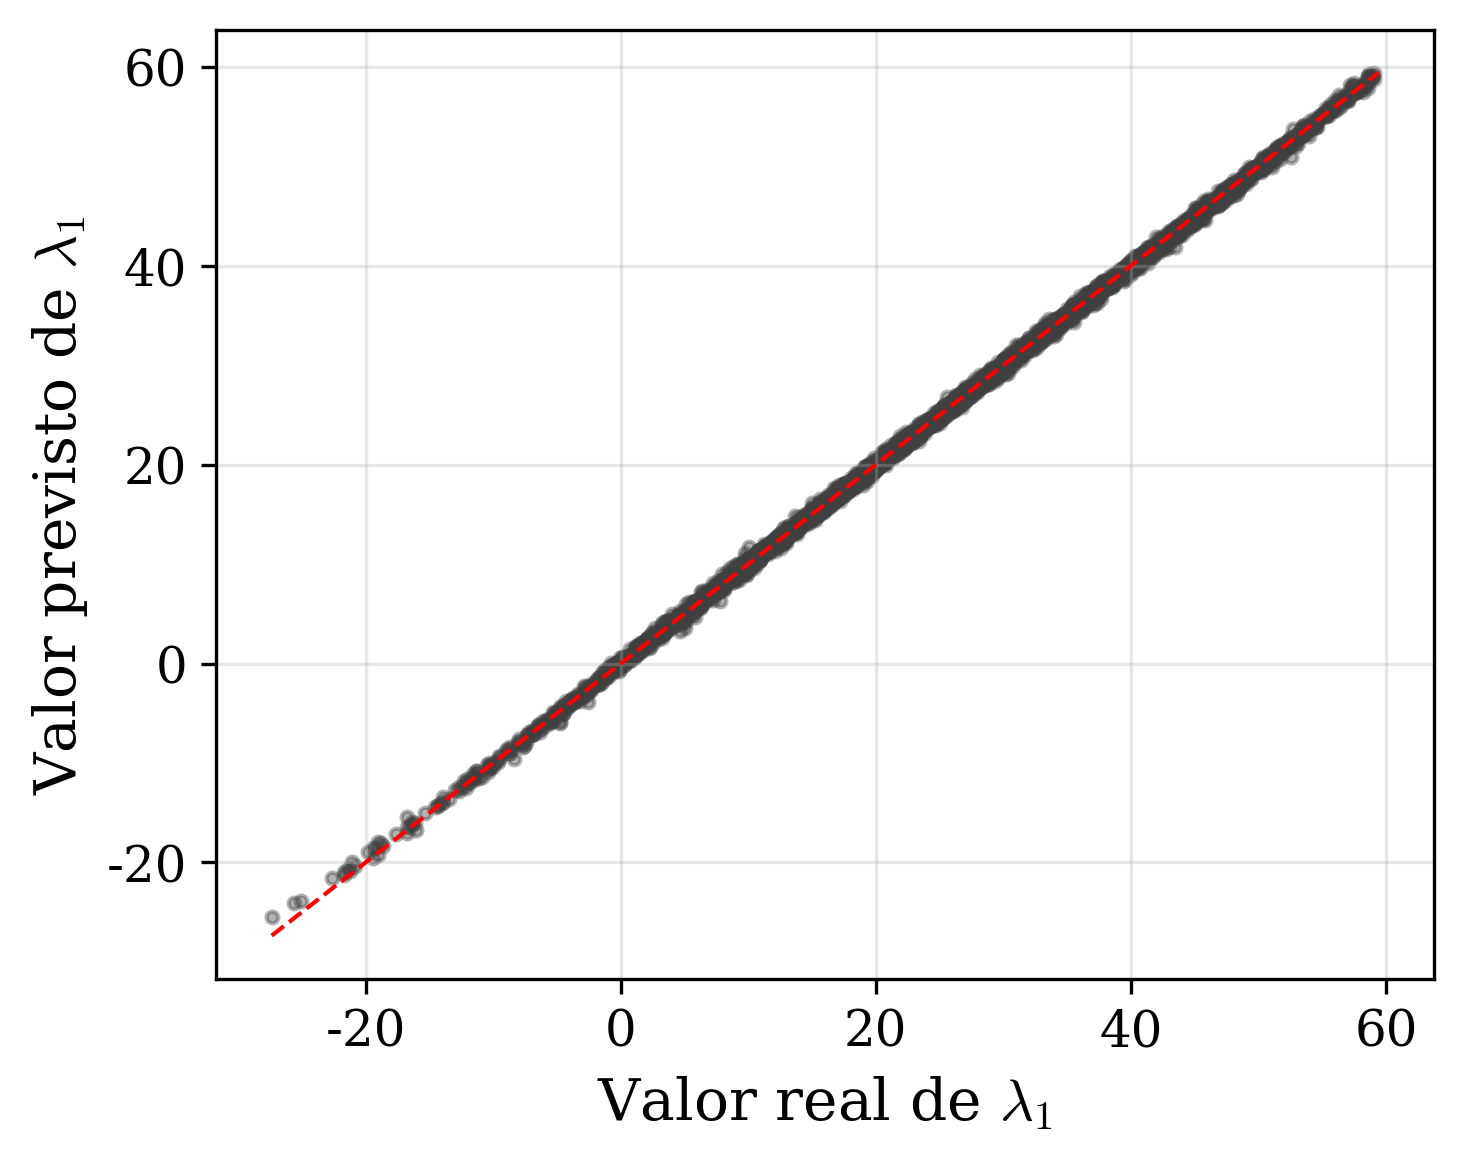
\includegraphics[width=\linewidth]{z_nn_pred_vs_true_lambda1_durability_pt.png}
        \caption{$\lambda_1$}
        \label{fig:nn_pred_vs_true_ex2_l1}
    \end{subfigure}
    \hfill
    \begin{subfigure}[b]{0.48\textwidth}
        \centering
        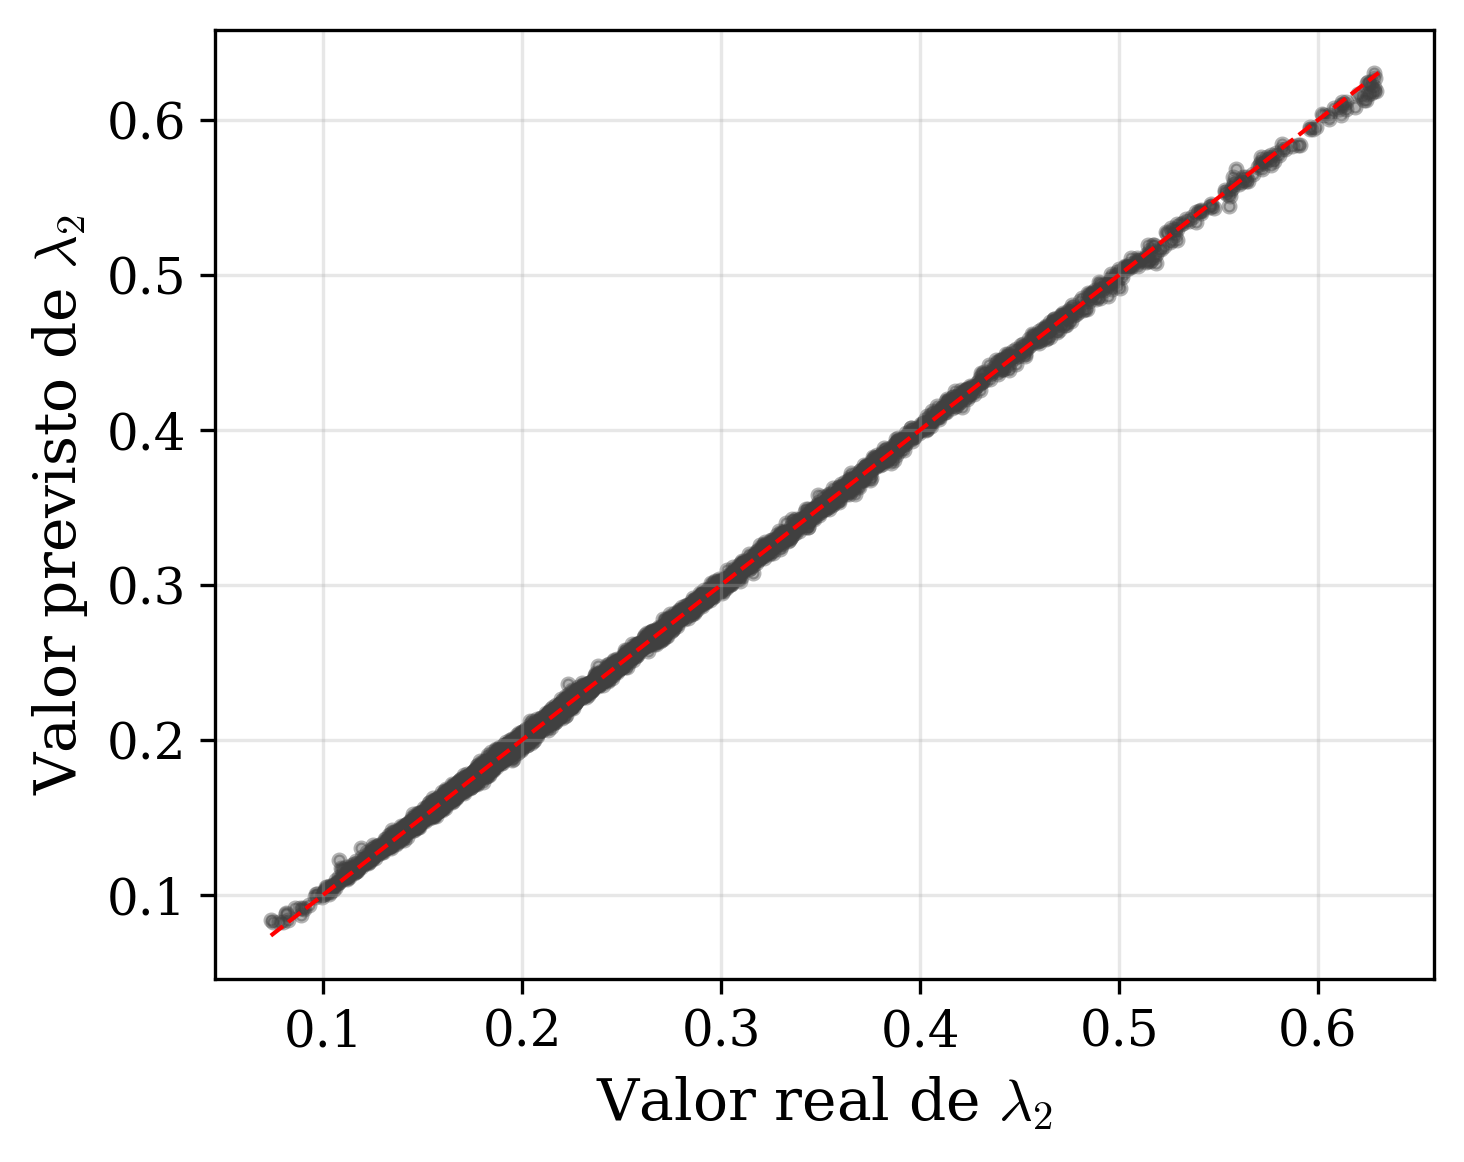
\includegraphics[width=\linewidth]{z_nn_pred_vs_true_lambda2_durability_pt.png}
        \caption{$\lambda_2$}
        \label{fig:nn_pred_vs_true_ex2_l2}
    \end{subfigure}
    \caption{Valor previsto versus valor real de $\lambda_1$ e $\lambda_2$ no conjunto de validação da rede neural global do Exemplo~2. A linha tracejada vermelha marca a identidade.}
    \label{fig:nn_pred_vs_true_ex2}
\end{figure}

\subsubsection{Comparação das distribuições e critérios de validação}

A avaliação distingue três níveis. No primeiro, os parâmetros previstos pela PCE são comparados aos ajustes locais nos $500$ pontos de validação em cada idade. No segundo, as redes são avaliadas na partição reservada da base gerada pelas PCEs. No terceiro, a distribuição reconstruída pelo emulador é comparada às amostras brutas de $g$ produzidas pelo simulador. Essa distinção é necessária porque um elevado $R^2$ da rede em relação às saídas da PCE mede a reprodução do metamodelo intermediário e pode coexistir com erro em relação à simulação física.

Os diagnósticos distribucionais configurados utilizam o primeiro ponto do conjunto de treinamento --- $f_c=30{,}805$~MPa, $UR=52{,}540\%$, $c_{\mathrm{nom}}=59{,}511$~mm --- nas idades de 50 e 100 anos, tanto para a PCE quanto para a rede. A comparação nas mesmas entradas facilita identificar o efeito da camada temporal, enquanto as duas idades permitem observar uma etapa intermediária e o final do horizonte. A referência é constituída pelas $2.500$ amostras brutas de $g$ desse ponto, e as métricas incluem KS, Wasserstein, divergência KL estimada por densidades suavizadas, $R^2$ entre densidades e erros nos quantis $P_5$, $P_{50}$ e $P_{95}$. Esses diagnósticos são verificações locais em idades de treinamento. A validação em idades intermediárias requer simulações diretas adicionais e não é realizada nesta execução.

\begin{table}[htbp]
\centering
\caption{Comparação distribucional do Exemplo~2 no ponto de projeto $f_c=30{,}805$~MPa, $UR=52{,}540\%$, $c_{\mathrm{nom}}=59{,}511$~mm.}
\label{tab:ex2_validacao}
\begin{tabular}{lcccc}
\toprule
 & \multicolumn{2}{c}{PCE} & \multicolumn{2}{c}{Rede neural} \\
\cmidrule(lr){2-3}\cmidrule(lr){4-5}
Métrica & 50 anos & 100 anos & 50 anos & 100 anos \\
\midrule
KS & 0,0232 & 0,0284 & 0,0300 & 0,0232 \\
Wasserstein (mm) & 0,4353 & 0,6952 & 0,5227 & 0,6933 \\
KL estimada & 0,01826 & 0,03487 & 0,02111 & 0,03245 \\
$R^2$ entre densidades & 0,99252 & 0,99232 & 0,99356 & 0,99204 \\
Erro relativo em $P_5$ (\%) & $-2{,}47$ & $+6{,}35$ & $-3{,}22$ & $+7{,}83$ \\
Erro relativo em $P_{50}$ (\%) & $+0{,}76$ & $-0{,}30$ & $+0{,}10$ & $+0{,}56$ \\
Erro relativo em $P_{95}$ (\%) & $-2{,}17$ & $-3{,}62$ & $-2{,}76$ & $-2{,}97$ \\
\bottomrule
\end{tabular}
\end{table}

\begin{figure}[H]
    \centering
    \begin{subfigure}[b]{0.48\textwidth}
        \centering
        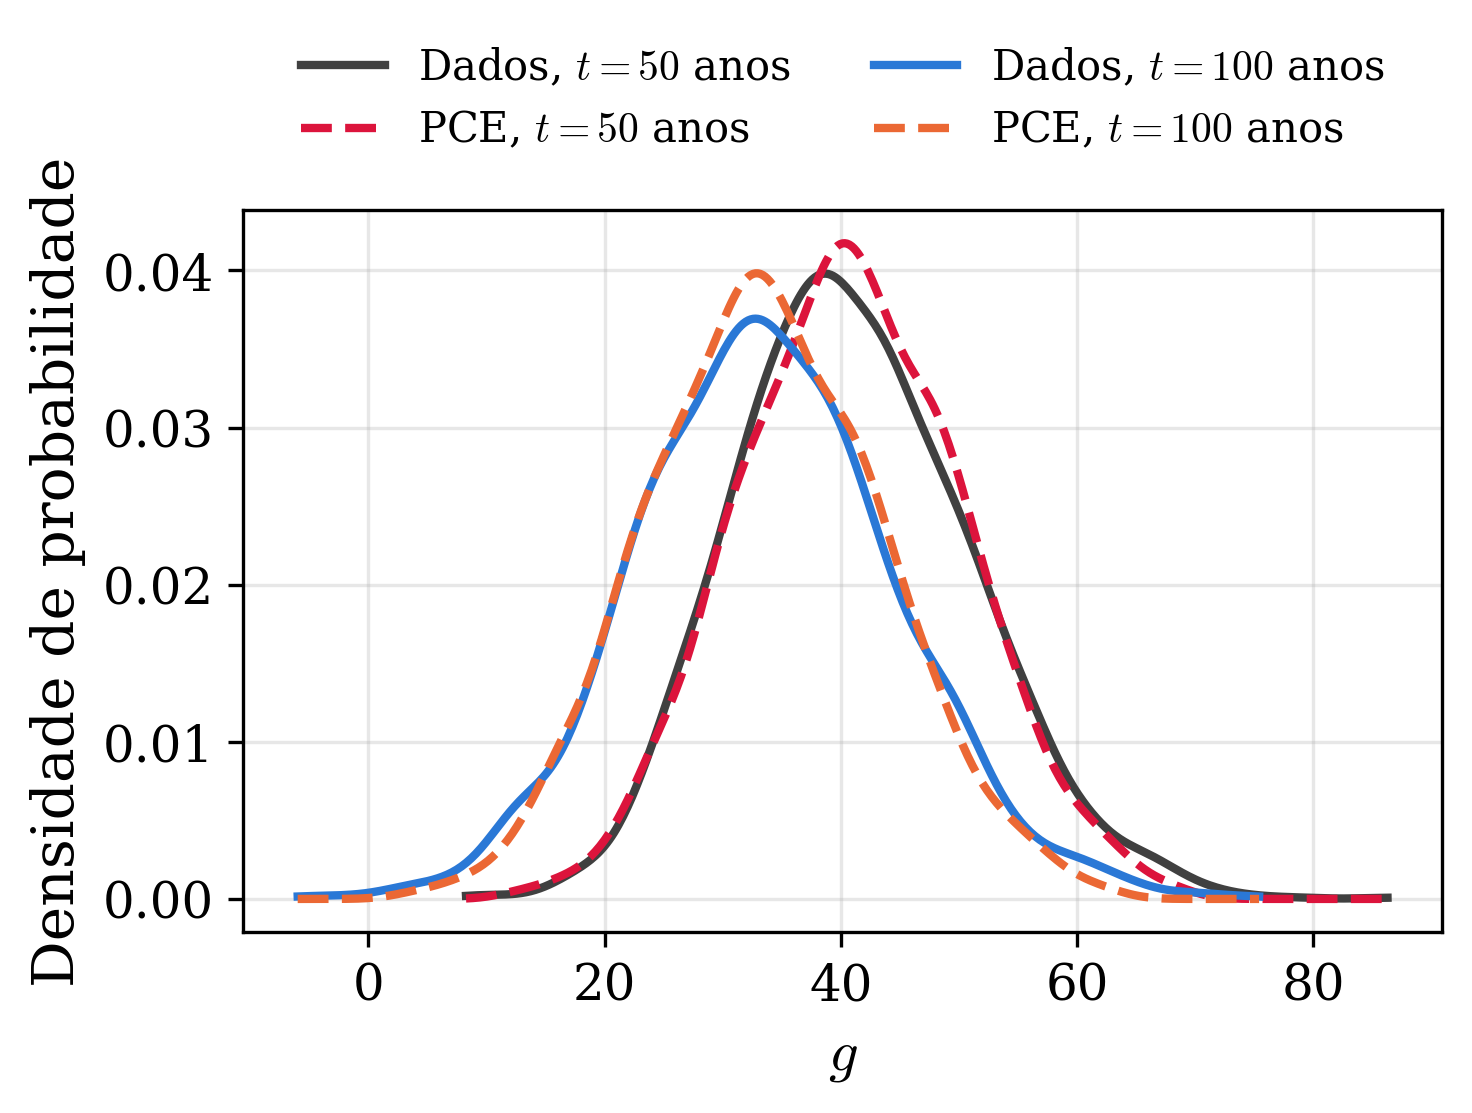
\includegraphics[width=\linewidth]{2500_kl_divergence_ex2_t50_vs_t100_pt.png}
        \caption{PCE}
        \label{fig:ex2_density_pce}
    \end{subfigure}
    \hfill
    \begin{subfigure}[b]{0.48\textwidth}
        \centering
        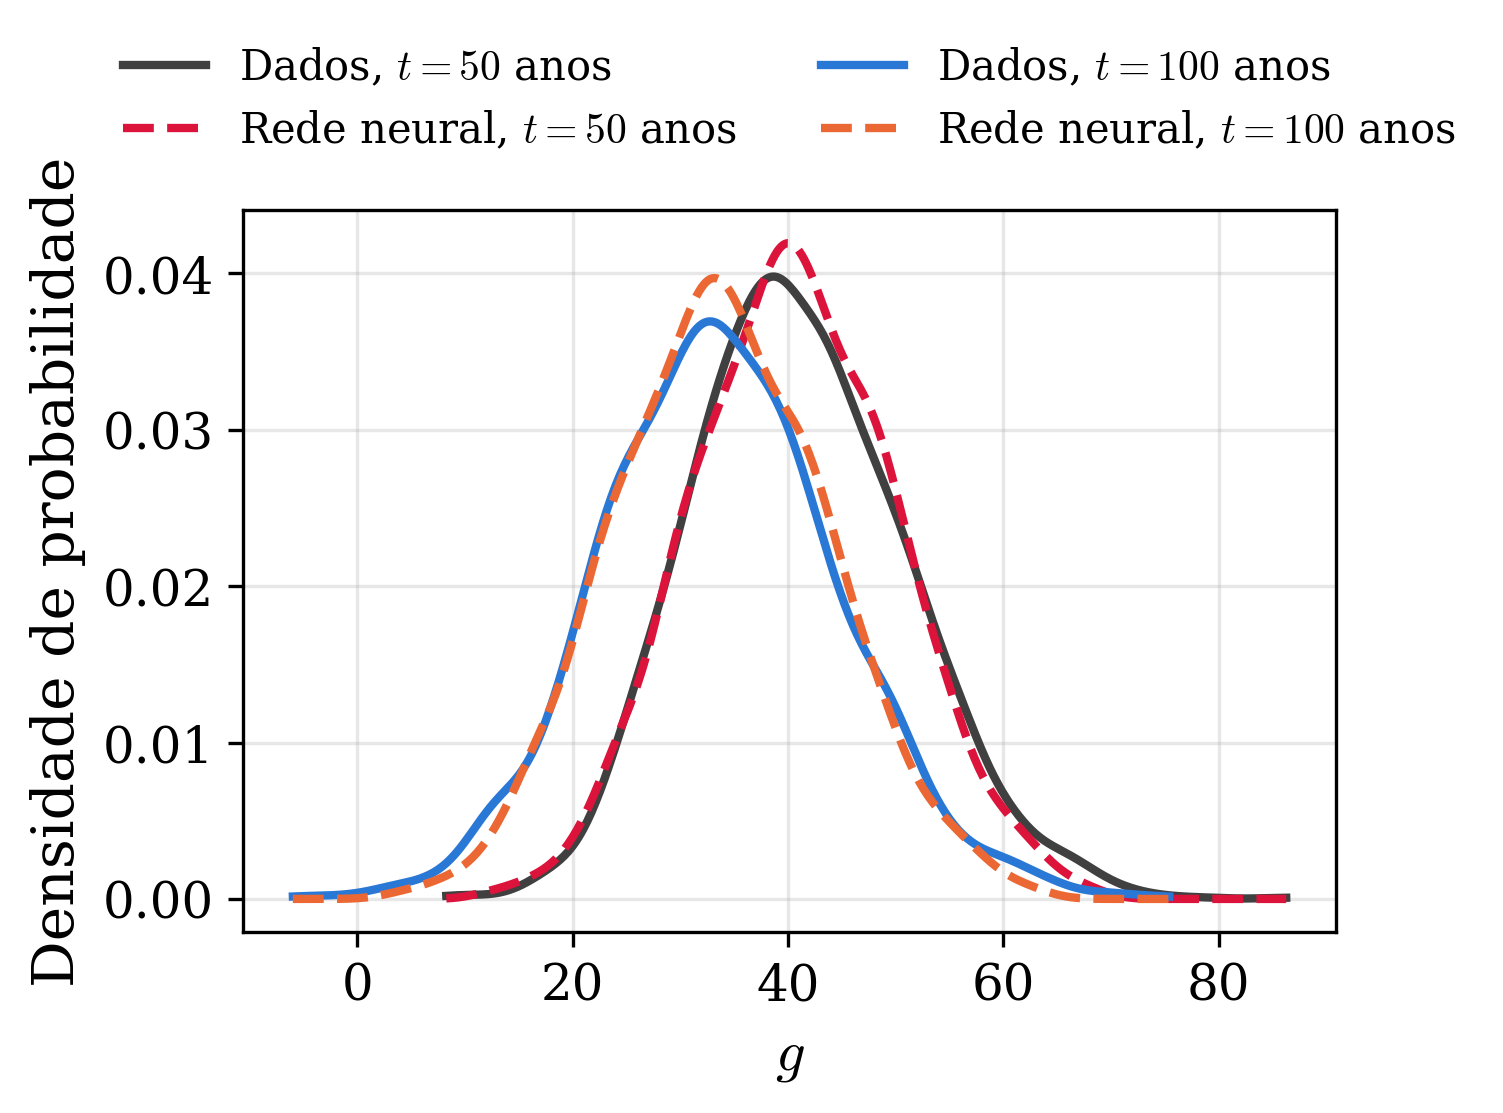
\includegraphics[width=\linewidth]{2500_nn_kl_divergence_ex2_t50_vs_t100_pt.png}
        \caption{Rede neural}
        \label{fig:ex2_density_nn}
    \end{subfigure}
    \caption{Densidades de referência (amostras brutas de $g$) e reconstruída pelo emulador, no ponto $f_c=30{,}805$~MPa, $UR=52{,}540\%$, $c_{\mathrm{nom}}=59{,}511$~mm, nas idades de 50 e 100 anos: PCE (esquerda) e rede neural (direita).}
    \label{fig:ex2_density_comparacao}
\end{figure}

Na Tabela~\ref{tab:ex2_validacao}, PCE e rede neural têm desempenho equivalente aos 50 anos, com $R^2$ acima de $0{,}992$ e erros de quantil abaixo de $3\%$ para ambas. Aos 100 anos, o comportamento reproduz o observado no Exemplo~\ref{subsec:exemplo1}: o erro relativo em $P_5$ cresce para os dois modelos --- $+6{,}35\%$ na PCE e $+7{,}83\%$ na rede neural ---, enquanto $P_{50}$ e $P_{95}$ permanecem abaixo de $4\%$. Ao contrário do problema de referência, aqui a rede neural não se distancia muito mais da PCE nessa cauda: a diferença entre os dois erros em $P_5$ aos 100 anos é de apenas $1{,}5$ pontos percentuais, contra dezenas de pontos no Exemplo~1. A Figura~\ref{fig:ex2_density_comparacao} mostra que, nas duas idades, a densidade reconstruída acompanha de perto a KDE das amostras brutas, com a maior discrepância concentrada na cauda inferior --- exatamente a região que determina a proximidade da despassivação. Como no Exemplo~1, a concordância no centro da distribuição não garante, isoladamente, a precisão da probabilidade de atingir um limiar preventivo baixo. A validação da interpolação temporal em idades não usadas no treinamento --- por exemplo, 40 ou 90 anos --- exigiria simulações diretas adicionais, não realizadas nesta execução.

\subsubsection{Trajetórias e vida remanescente no ponto fixado}

No ponto da Tabela~\ref{tab:viga_va}, a rede é consultada em 20 idades igualmente espaçadas entre zero e 100 anos, com intervalo aproximado de $5{,}26$ anos. São geradas $50.000$ trajetórias por acoplamento quantílico: cada trajetória mantém o mesmo nível uniforme $u_i$ ao avaliar $g_i(t)=Q(u_i;\hat{\boldsymbol{\lambda}}(t))$. As $50.000$ amostras reduzem a variabilidade do pós-processamento da GLD; não aumentam a informação física disponível para treinar o emulador. Para a visualização das trajetórias são utilizadas apenas 300 delas.

O acoplamento preserva a posição relativa de cada realização entre as distribuições, estabelecendo uma hipótese explícita de dependência temporal. A monotonicidade física da profundidade no simulador não garante que todas as curvas quantílicas da rede sejam monotônicas. Por isso, a interpretação em termos de primeira passagem exige verificar a evolução das trajetórias emuladas. Consultar 20 idades, em vez das cinco usadas no treinamento, permite localizar o cruzamento com maior resolução, mas a precisão desse refinamento depende da interpolação aprendida.

A configuração principal considera $g_{\mathrm{lim}}=5$~mm. Nesse caso, o tempo calculado representa o prazo até que restem 5~mm de cobrimento não carbonatado. O instante de cruzamento é estimado por interpolação linear entre as duas idades adjacentes que o delimitam. O caso $g_{\mathrm{lim}}=0$, incluído no Exemplo~3, fornece a referência correspondente à despassivação. Assim, a interpretação da vida remanescente sempre deve ser acompanhada do limiar que define o evento.

A avaliação condicional adota $t_{\mathrm{insp}}=25$ anos, correspondente a 2005, para representar a análise de um elemento após parte de sua exposição. Consideram-se as trajetórias que ainda não atingiram o limiar nessa idade, e a vida remanescente é medida a partir dela, conforme a Equação~\eqref{eq:rul}. Como 25 anos não pertence à malha de 20 idades do pós-processamento, a margem nesse instante também é obtida por interpolação. Esse condicionamento usa apenas a informação de que o limiar ainda não foi alcançado; uma atualização baseada em medições de carbonatação exigiria incorporar dados de inspeção.

As trajetórias que não atingem o limiar até 100 anos são censuradas à direita. O horizonte disponível a partir de $t_{\mathrm{insp}}=25$ anos é, portanto, de 75 anos. Uma concentração de valores nesse limite nos gráficos resulta da convenção numérica de encerrar a observação, e não da identificação de uma vida útil exatamente igual a 75 anos. A média calculada mantendo esses valores é uma média restrita ao horizonte, enquanto os quantis que recaem na região censurada não são determinados pela simulação.

Ao longo das 20 idades consultadas nesse ponto, $\lambda_2$ permanece positivo, decrescendo de $0{,}393$ em $t=0$ a $0{,}146$ em $t=100$ anos, o que garante uma GLD válida em toda a trajetória. Em $t=0$ nenhuma das $50.000$ realizações está abaixo do limiar de 5~mm --- a média de $g$ nessa idade é $24{,}95$~mm, com $P(g\leq5)=0$ ---, de modo que todo cruzamento observado corresponde a uma primeira passagem genuína, sem trajetórias que já iniciem abaixo do limiar.

\begin{figure}[H]
    \centering
    \begin{subfigure}[b]{0.48\textwidth}
        \centering
        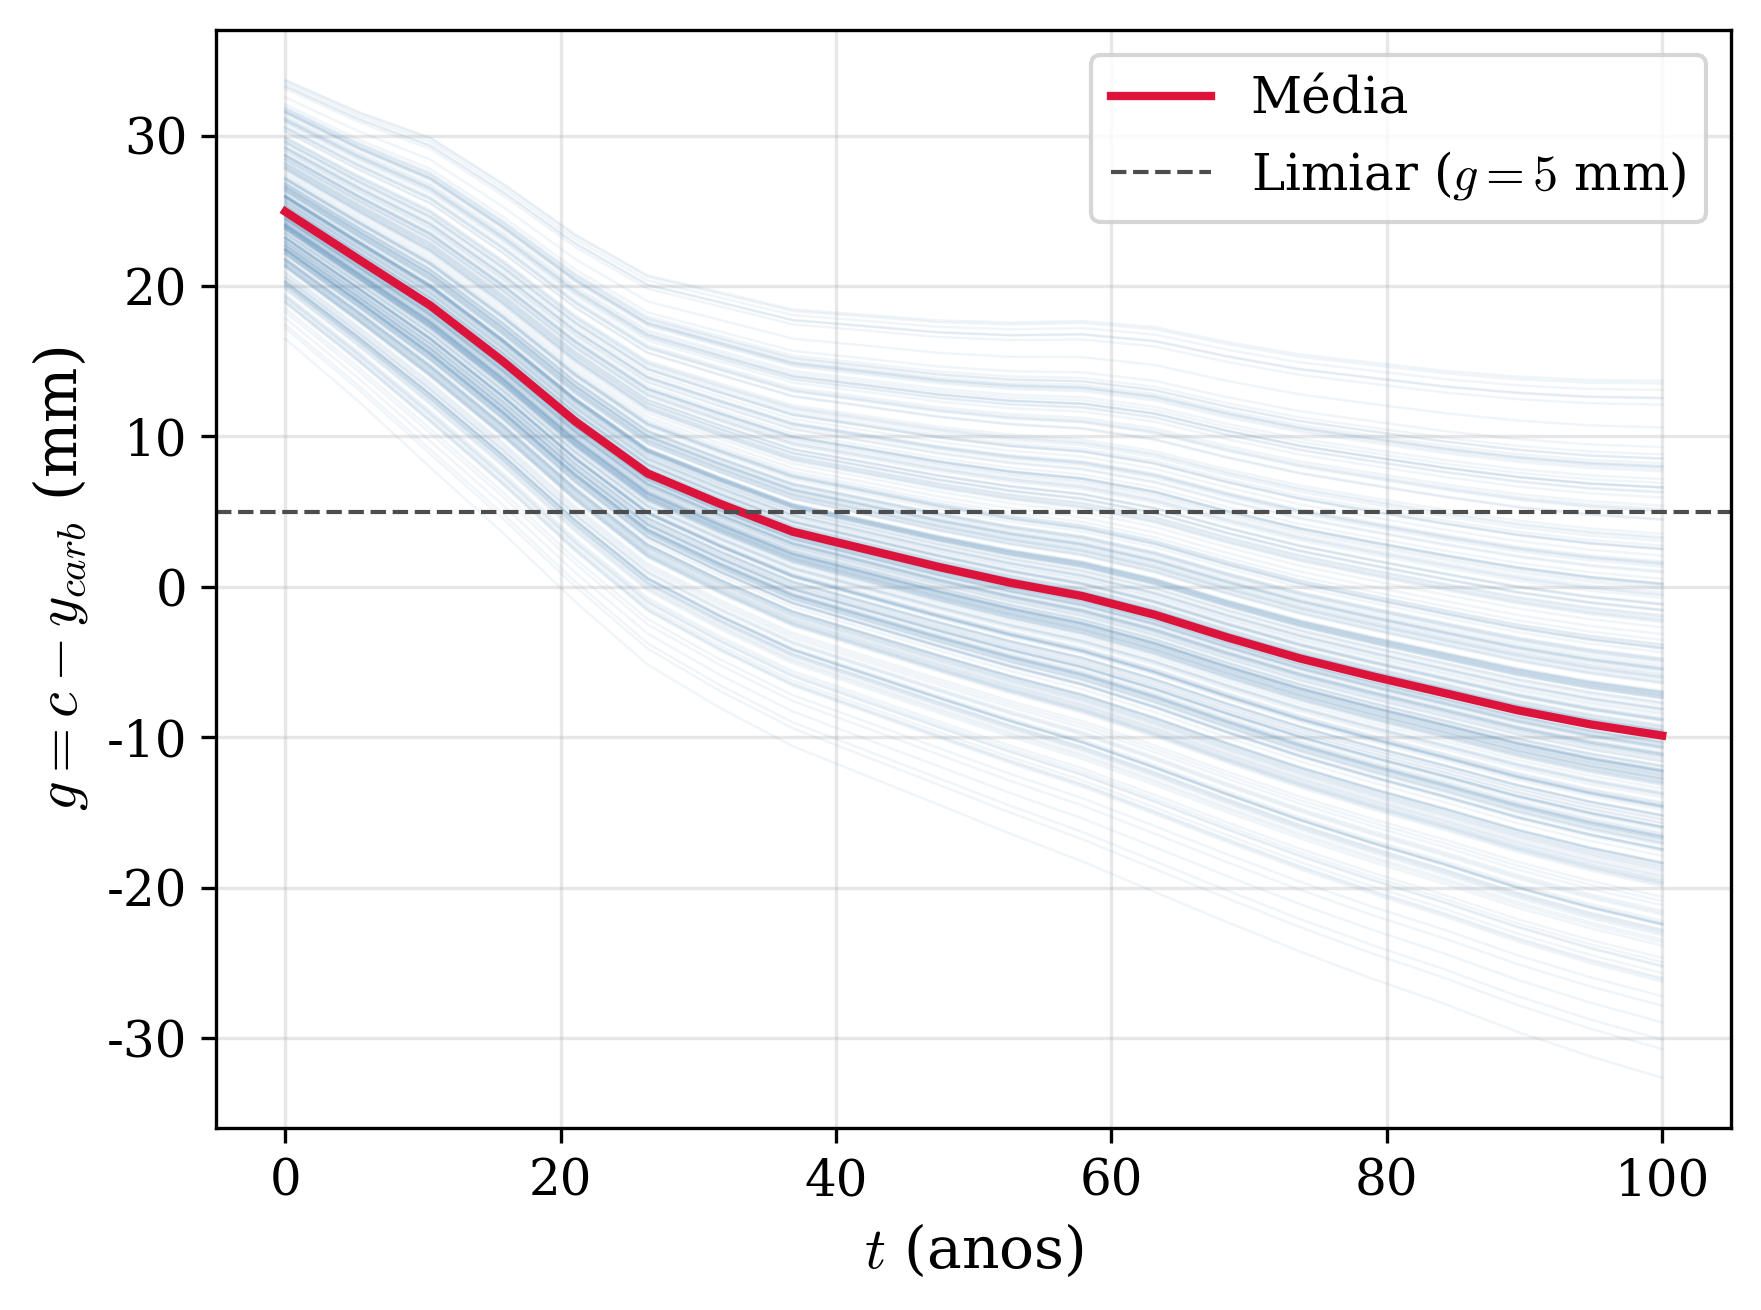
\includegraphics[width=\linewidth]{2500_rul_samples_fck25_rh55_cov25_durability_spaghetti_pt.png}
        \caption{Trajetórias de $g(t)$.}
        \label{fig:ex2_rul_spaghetti}
    \end{subfigure}
    \hfill
    \begin{subfigure}[b]{0.48\textwidth}
        \centering
        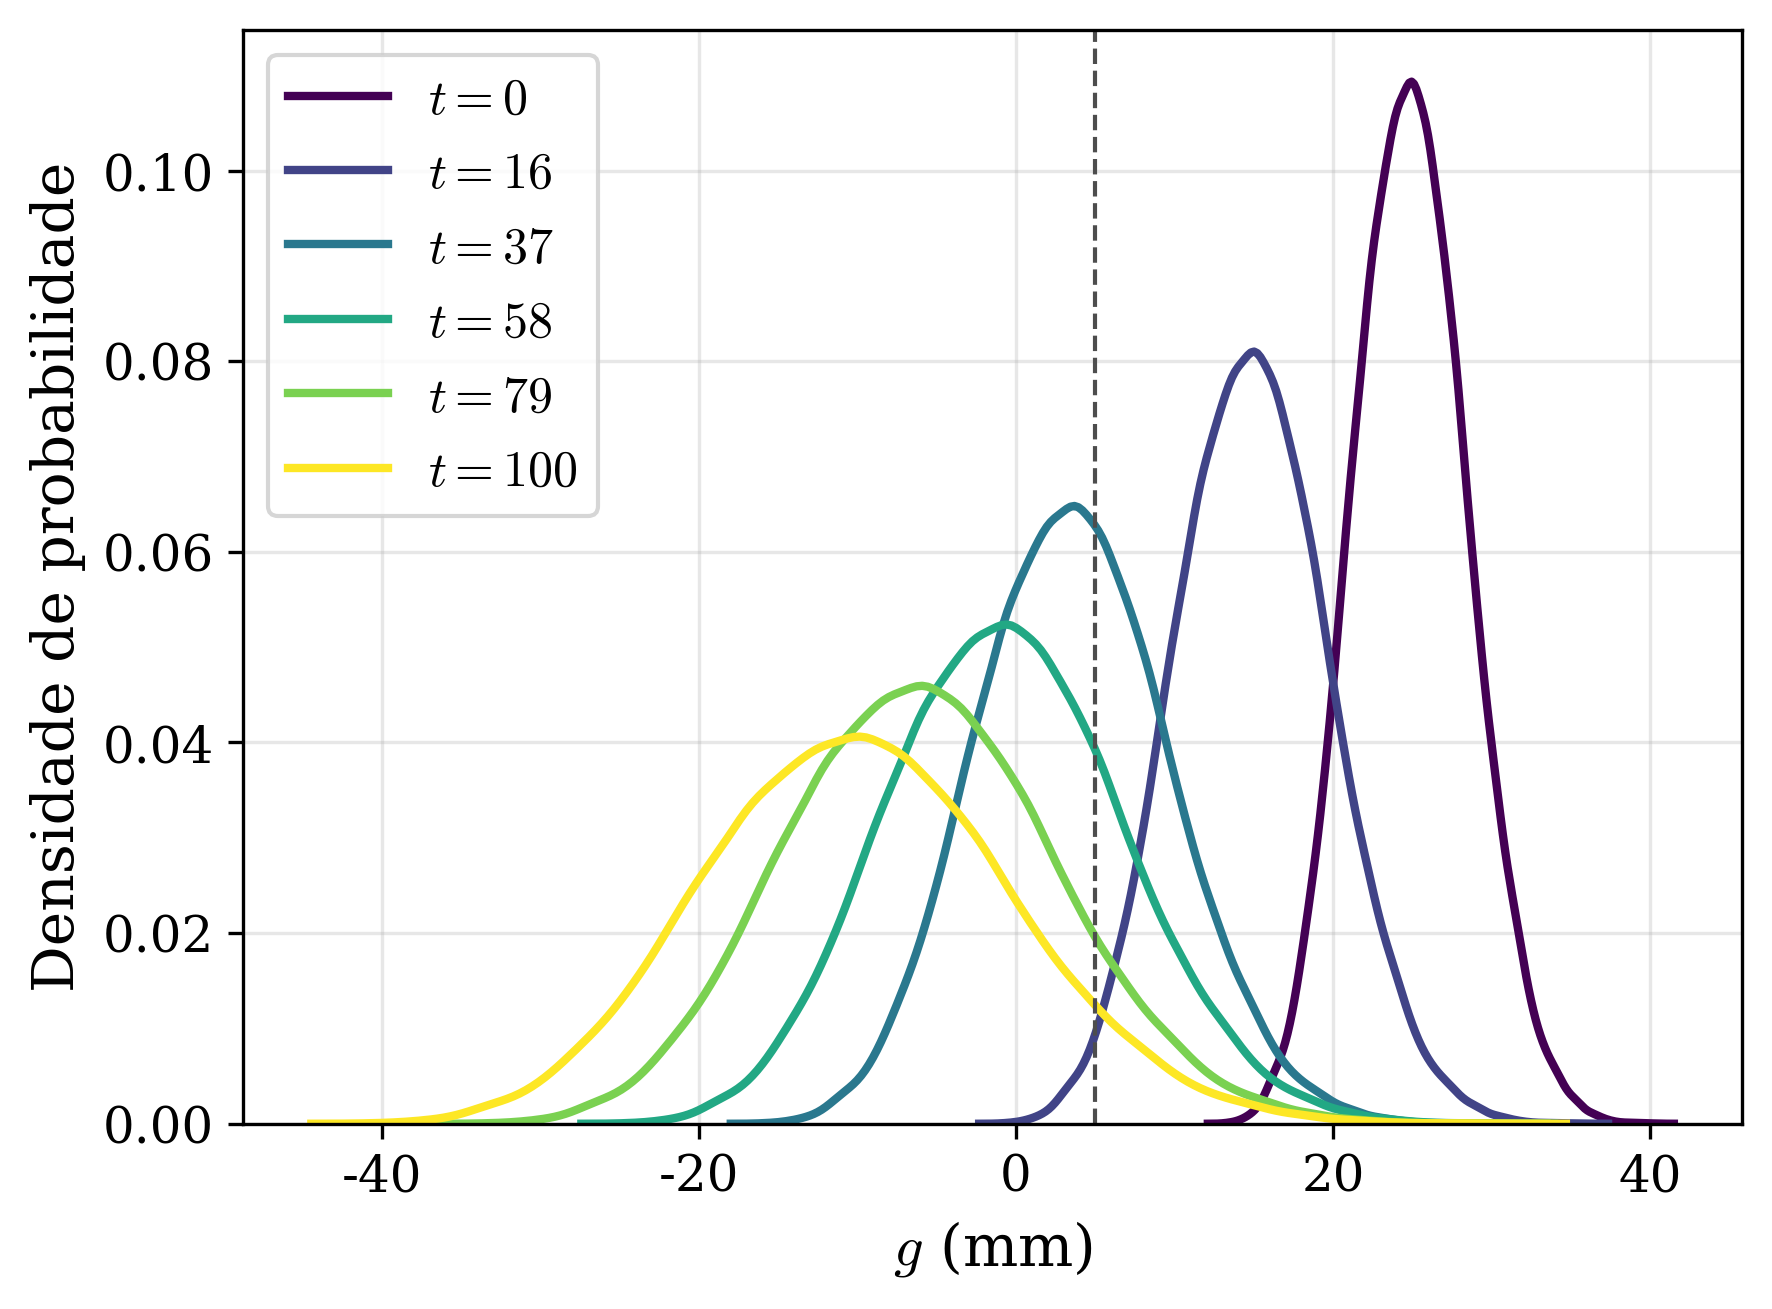
\includegraphics[width=\linewidth]{2500_rul_samples_fck25_rh55_cov25_durability_g_pdfs_pt.png}
        \caption{Densidade de $g$ em seis idades.}
        \label{fig:ex2_rul_g_pdfs}
    \end{subfigure}
    \caption{Comportamento de $g(t)$ no ponto $f_c=25$~MPa, $UR=55\%$, $c_{\mathrm{nom}}=25$~mm: (a) $300$ das $50.000$ trajetórias emuladas pela rede, com a média (vermelho); (b) densidade de $g$ em seis idades entre $0$ e $100$ anos. O limiar de intervenção $g=5$~mm é indicado em ambos os painéis (tracejado).}
    \label{fig:ex2_rul_trajetorias}
\end{figure}

A dispersão entre trajetórias cresce com o tempo, e a média cruza o limiar de 5~mm por volta de $t=33$ anos (Figura~\ref{fig:ex2_rul_trajetorias}a). Do total de $50.000$ trajetórias, $3.279$ ($6{,}56\%$) não atingem o limiar dentro do horizonte de 100 anos e são censuradas à direita. Entre as $46.721$ que cruzam, o tempo até o limiar tem média de $41{,}70$ anos, mediana de $32{,}74$ anos, desvio padrão de $23{,}52$ anos e $P_5=18{,}46$ anos; o $P_{95}$ empírico da amostra completa recai no limite do horizonte ($100$ anos), refletindo a fração censurada.

\begin{figure}[H]
    \centering
    \begin{subfigure}[b]{0.48\textwidth}
        \centering
        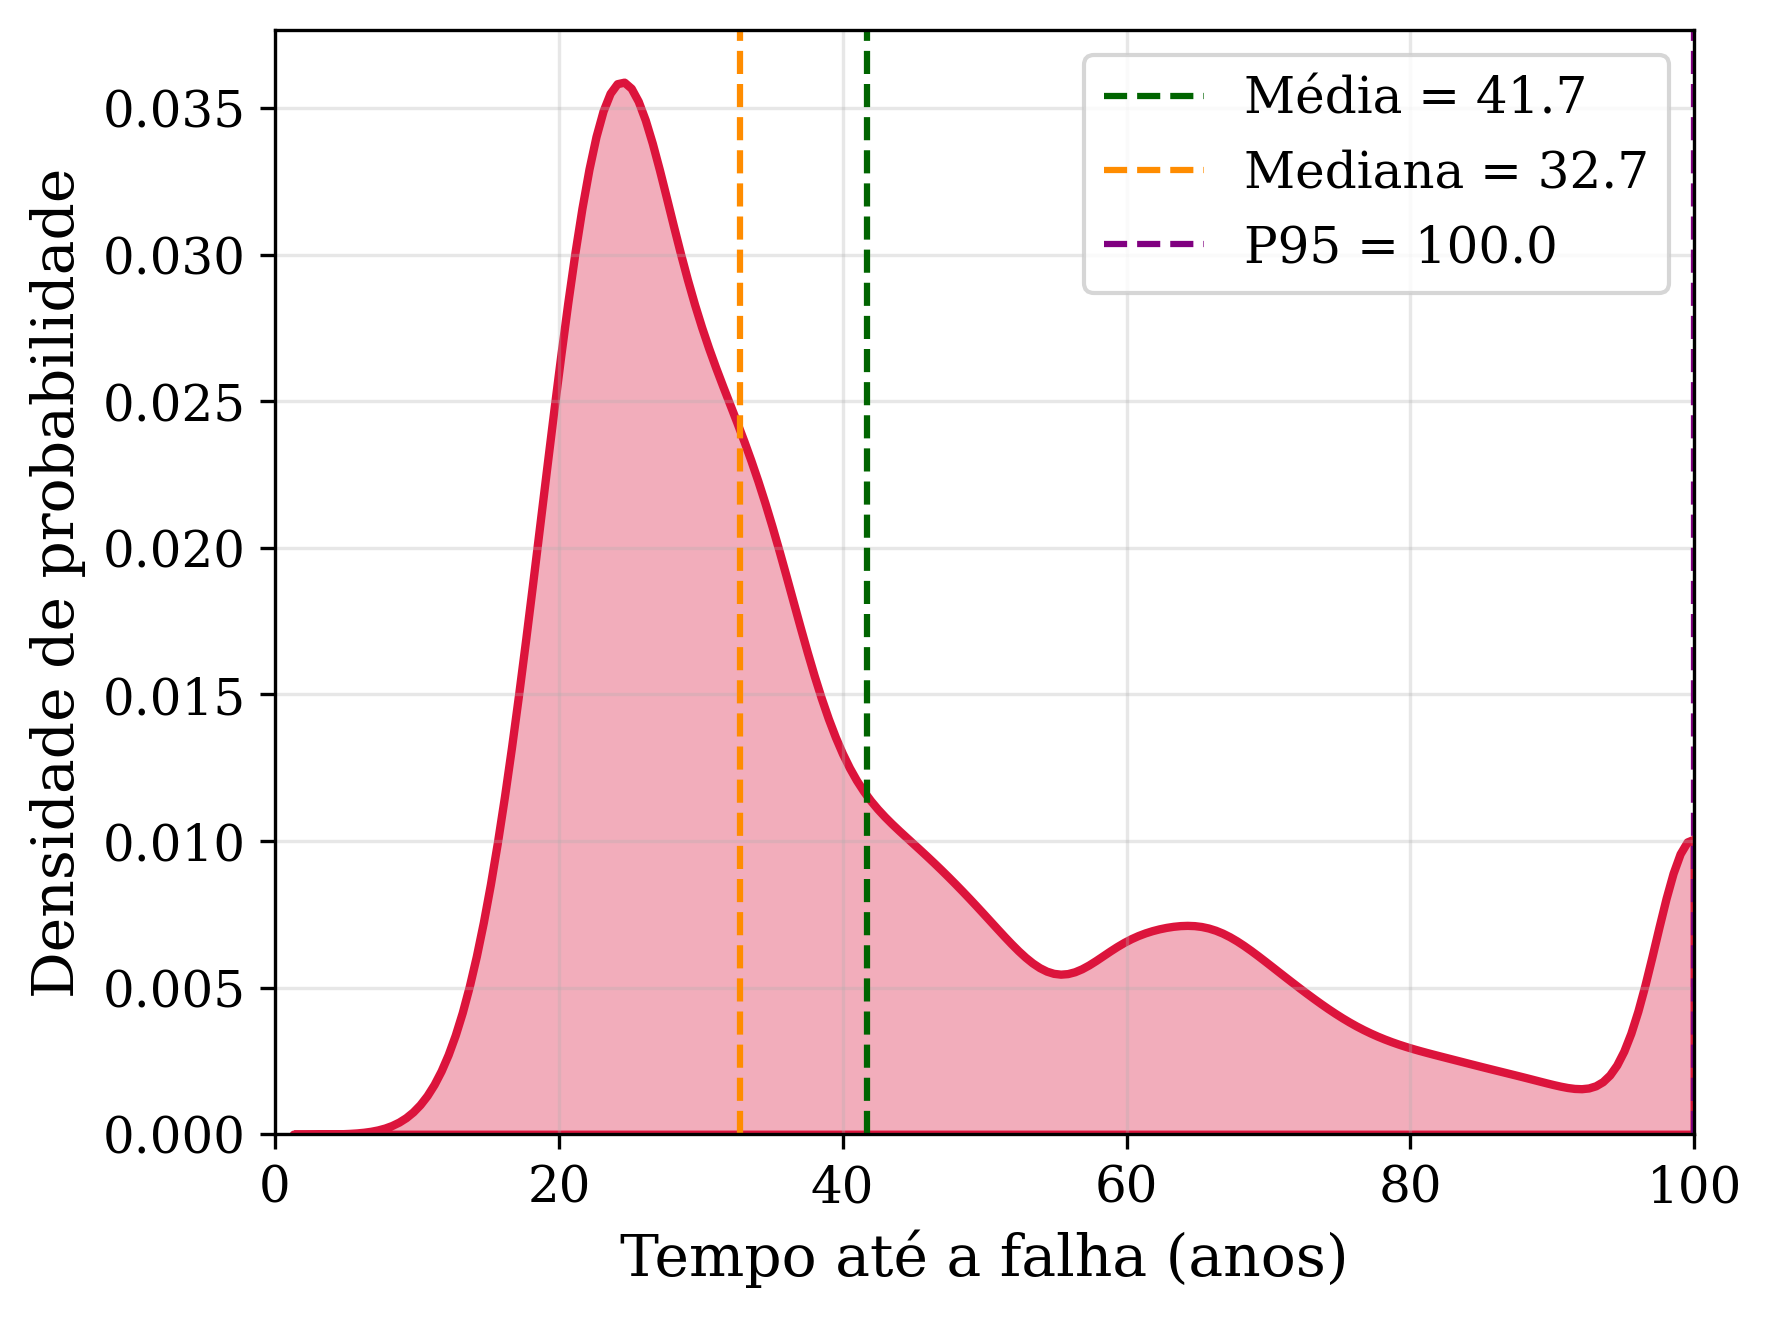
\includegraphics[width=\linewidth]{2500_rul_samples_fck25_rh55_cov25_durability_rul_pdf_pt.png}
        \caption{Tempo até o cruzamento, a partir de $t=0$.}
        \label{fig:ex2_rul_pdf}
    \end{subfigure}
    \hfill
    \begin{subfigure}[b]{0.48\textwidth}
        \centering
        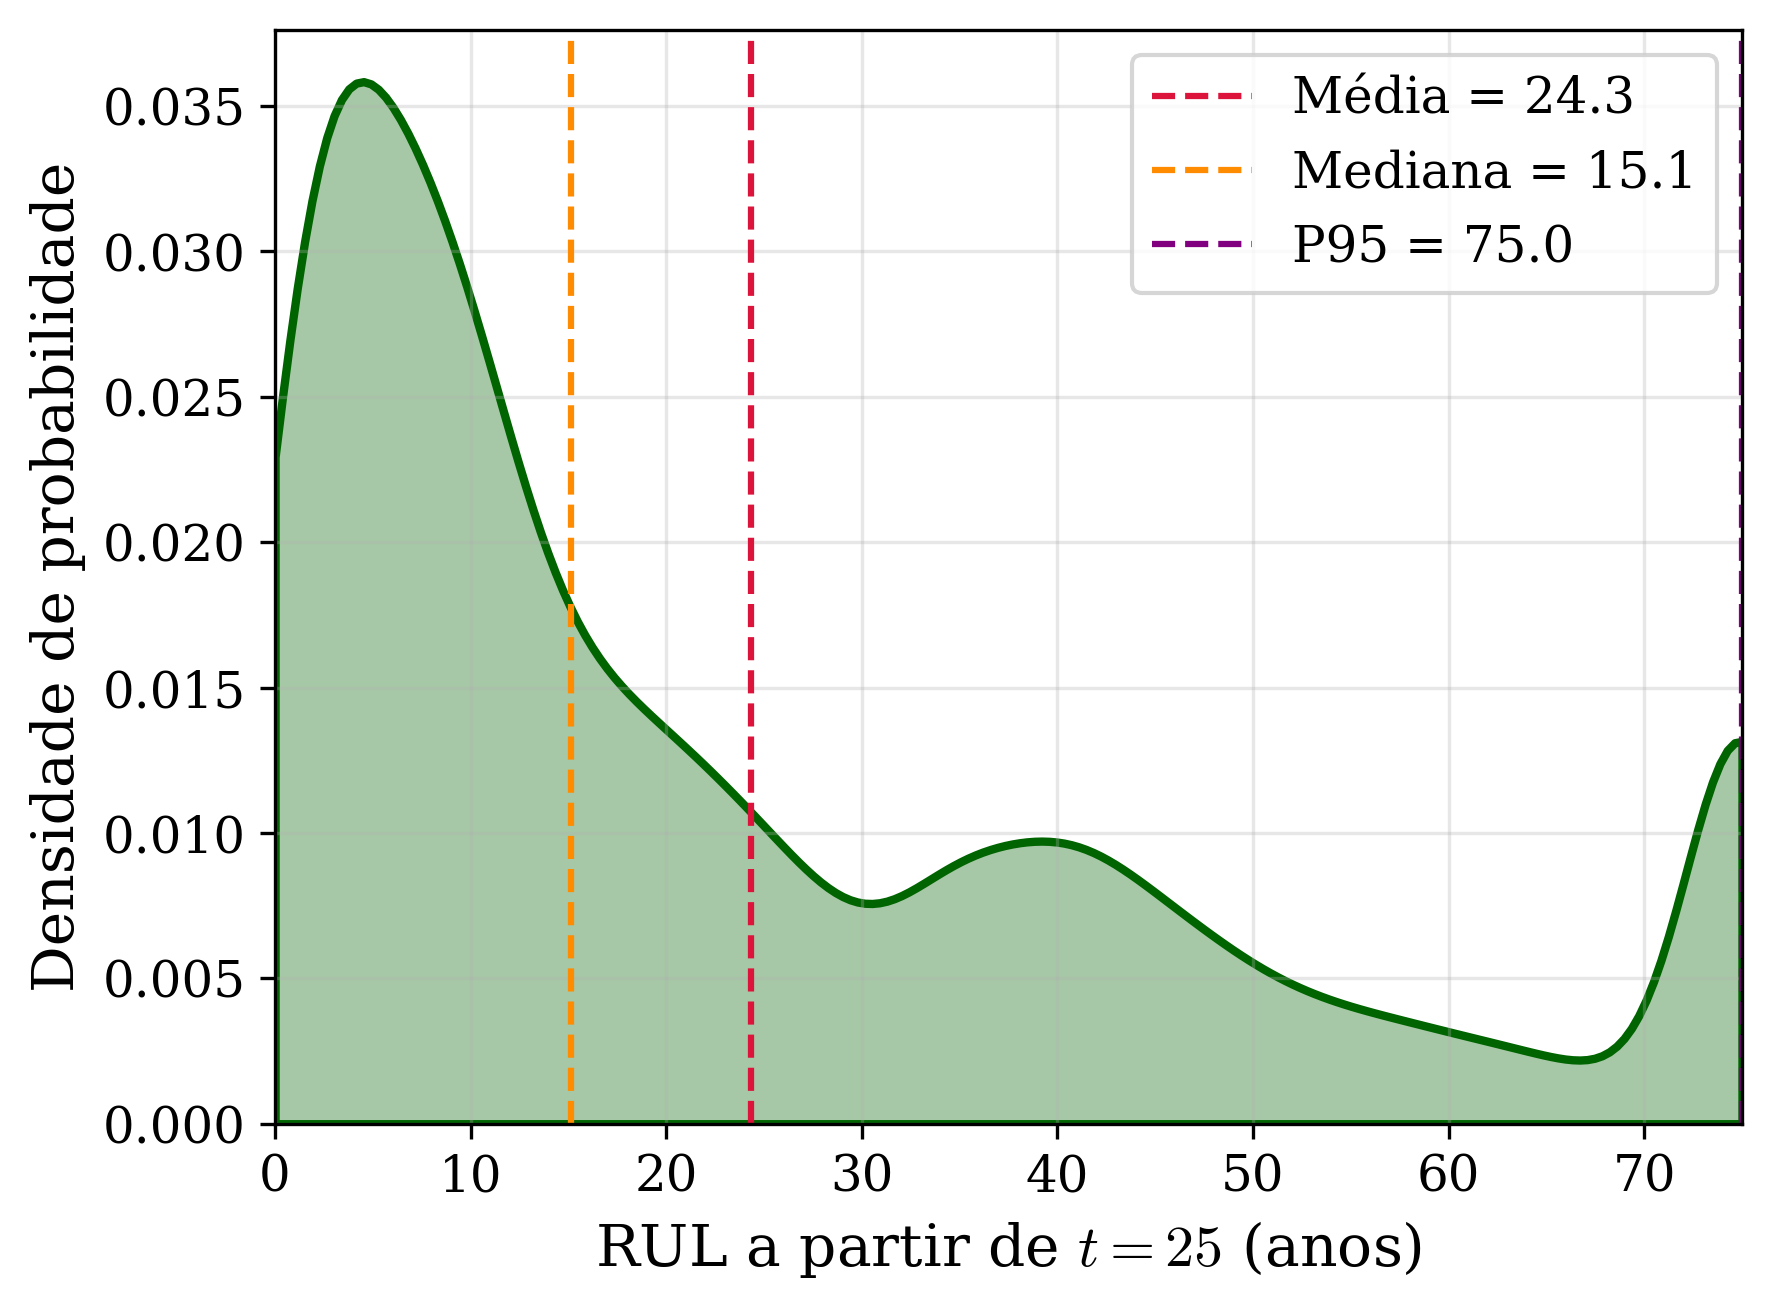
\includegraphics[width=\linewidth]{2500_rul_samples_fck25_rh55_cov25_durability_conditional_rul_t25_pt.png}
        \caption{RUL condicionada à sobrevivência em $t=25$ anos.}
        \label{fig:ex2_rul_conditional}
    \end{subfigure}
    \caption{Distribuição do tempo até o cruzamento do limiar $g=5$~mm, no ponto $f_c=25$~MPa, $UR=55\%$, $c_{\mathrm{nom}}=25$~mm: (a) a partir de $t=0$; (b) vida útil remanescente condicionada à sobrevivência em $t_{\mathrm{insp}}=25$ anos. Ambas as densidades são truncadas no maior valor alcançável dentro do horizonte simulado de 100 anos.}
    \label{fig:ex2_rul_distribuicoes}
\end{figure}

Em $t_{\mathrm{insp}}=25$ anos, $36.509$ das $50.000$ trajetórias ($73{,}02\%$) ainda não atingiram o limiar; as demais $13.491$ ($26{,}98\%$) já o haviam cruzado antes dessa idade e ficam fora do condicionamento. Para as sobreviventes, a RUL medida a partir de $t=25$ anos (Figura~\ref{fig:ex2_rul_distribuicoes}b) tem média de $24{,}32$ anos, mediana de $15{,}15$ anos e $P_{95}=75{,}00$ anos --- novamente no limite do horizonte disponível a partir dessa idade ($100-25=75$ anos), de modo que o percentil 95 da RUL condicional completa não é determinado pela simulação. A diferença entre a média ($24{,}32$ anos) e a mediana ($15{,}15$ anos) reflete a assimetria à direita introduzida pela censura: a cauda longa de trajetórias que só cruzam o limiar perto do fim do horizonte, ou nunca o cruzam, eleva a média sem deslocar igualmente a mediana.

\subsubsection{Custo computacional}

A avaliação de custo segue a definição da Equação~\eqref{eq:ex1_speedup}: em cada idade, compara-se o tempo de geração das réplicas, organização dos dados e ajuste local da GLD com o tempo de predição da PCE no mesmo lote de $2.000$ entradas. Essa razão caracteriza o custo de obtenção dos parâmetros distribucionais. O treinamento das PCEs e das redes, a amostragem das trajetórias e o cálculo dos cruzamentos são etapas distintas e devem ser reportadas separadamente quando se avaliar o custo total.

\begin{table}[H]
\centering
\caption{Tempos por lote de pontos de projeto e ganho computacional nas cinco idades avaliadas, no Exemplo~2.}
\label{tab:computational_time_ex2}
\begin{tabular}{rrrr}
\toprule
Tempo (anos) & Referência (s) & Emulador PCE (s) & Ganho (vezes) \\
\midrule
0,00   & 362,077174 & 0,006031 & 60.039 \\
25,00  & 366,391805 & 0,005807 & 63.092 \\
50,00  & 358,595040 & 0,005823 & 61.582 \\
75,00  & 357,628061 & 0,002588 & 138.163 \\
100,00 & 358,440037 & 0,002412 & 148.633 \\
\midrule
Mediana & 358,595040 & 0,005807 & 63.092 \\
\bottomrule
\end{tabular}
\par\smallskip
\begin{minipage}{0.92\linewidth}
\footnotesize A última linha apresenta a mediana de cada coluna, calculada como no Exemplo~1: a mediana do ganho é a mediana das cinco razões, não a razão entre os tempos medianos.
\end{minipage}
\end{table}

O procedimento de referência --- que inclui a geração das réplicas latentes, a avaliação do modelo de carbonatação e o ajuste local da GLD --- demandou, na mediana, $358{,}60$~s por idade, contra aproximadamente $5{,}81$~ms da predição pela PCE já treinada. A mediana dos ganhos foi de $6{,}31\times10^4$ vezes, com valores entre $6{,}00\times10^4$ (t=0) e $1{,}49\times10^5$ (t=100). Esse ganho é uma ordem de grandeza menor que o do Exemplo~1 ($5{,}57\times10^5$), coerente com o registro disponível conter apenas uma cronometragem por idade, sem repetições, e não deve ser interpretado como uma medida mais precisa da eficiência da PCE em si.

Chama atenção a diferença entre os tempos de predição da PCE em $t=0$, $25$ e $50$ anos (entre $5{,}8$ e $6{,}0$~ms) e em $t=75$ e $100$ anos (entre $2{,}4$ e $2{,}6$~ms), aproximadamente $2{,}3$ vezes menores. Como a arquitetura da PCE --- grau total três, 20 termos por parâmetro --- é a mesma em todas as idades, essa diferença é atribuída a variações no ambiente de execução durante a cronometragem (por exemplo, estado do cache ou de outros processos), e não a uma diferença estrutural do modelo entre idades; a ausência de repetições impede quantificar essa variabilidade. Ainda assim, mesmo no cenário mais conservador ($t=0$), a consulta ao emulador é cerca de $6\times10^4$ vezes mais rápida que o procedimento de referência, o que favorece decisivamente a avaliação repetida de cenários --- por exemplo, a varredura de limiares do Exemplo~\ref{subsec:exemplo3} ou análises de sensibilidade que exijam milhares de consultas --- frente ao custo de construir o emulador uma única vez. O treinamento das PCEs e da camada temporal, bem como a amostragem das $50.000$ trajetórias e o cálculo dos cruzamentos da Seção anterior, não estão incluídos nesta comparação e representam um custo fixo, pago uma vez, que se dilui à medida que o emulador é reutilizado.

% =====================================================================
\subsection{Exemplo 3: efeito do limiar de manutenção preventiva}
\label{subsec:exemplo3}

O terceiro exemplo utiliza o elemento e as trajetórias do Exemplo~2 para examinar como o critério de intervenção modifica a distribuição do tempo disponível para manutenção. Mantêm-se o ponto de projeto, o cenário ambiental e as variáveis latentes, variando-se apenas $g_{\mathrm{lim}}$. Essa escolha permite associar as diferenças entre os prazos à política adotada.

\subsubsection{Definição e justificativa dos limiares}

São considerados $g_{\mathrm{lim}}\in\{0,2,5,8,12\}$~mm, conforme a configuração da análise de RUL. O limiar nulo corresponde à despassivação e estabelece a referência física da comparação. Os valores positivos representam margens preventivas crescentes: quanto maior o limiar, menor o avanço da frente carbonatada admitido antes da intervenção. O valor de 5~mm mantém a configuração principal do Exemplo~2, enquanto os demais permitem observar o efeito de reduzir ou ampliar essa margem. Esses valores são parâmetros de um estudo de políticas e não limites prescritos por norma.

Para uma mesma realização com cobrimento efetivo $c_i$, o limiar equivale a admitir uma profundidade $y_{\mathrm{lim},i}=c_i-g_{\mathrm{lim}}$. A Tabela~\ref{tab:ex3_limiares} apresenta essa relação para o cobrimento nominal de 25~mm; nas simulações, a variabilidade de $c_i$ é preservada. A apresentação em milímetros mantém uma ligação direta com a grandeza física que poderia ser avaliada em uma inspeção.

\begin{table}[htbp]
\centering
\caption{Interpretação dos limiares de intervenção para o cobrimento nominal de 25~mm.}
\label{tab:ex3_limiares}
\begin{tabular}{ccl}
\toprule
$g_{\mathrm{lim}}$ (mm) & $c_{\mathrm{nom}}-g_{\mathrm{lim}}$ (mm) & Interpretação \\
\midrule
0 & 25 & Referência de despassivação \\
2 & 23 & Margem preventiva de 2~mm \\
5 & 20 & Política principal do Exemplo~2 \\
8 & 17 & Margem preventiva de 8~mm \\
12 & 13 & Margem preventiva de 12~mm \\
\bottomrule
\end{tabular}
\end{table}

Para cada trajetória calcula-se o primeiro cruzamento de cada limiar, conforme a Seção~\ref{subsec:manutencao}. A reutilização das mesmas realizações permite uma comparação pareada das políticas e dispensa novas consultas ao modelo físico. Para trajetórias inicialmente acima dos limiares, o tempo de cruzamento de um limiar maior é menor ou igual ao de um limiar menor. Essa ordenação fornece uma verificação de coerência do pós-processamento. Se uma trajetória já se encontra abaixo de um limiar no início da observação, o evento deve ser identificado como já ocorrido.

\subsubsection{Comparação dos prazos e tratamento da censura}

A comparação inclui a proporção de trajetórias que atingem cada limiar durante o horizonte, a proporção censurada e as estatísticas do tempo até o cruzamento. A Tabela~\ref{tab:ex3_cenarios} segue o resumo configurado no notebook: média, $P_5$ e mediana são calculados apenas entre as trajetórias cujo cruzamento é identificado antes do final do horizonte.

\begin{table}[htbp]
\centering
\caption{Tempo até os limiares preventivos, contado a partir do início da exposição. As estatísticas de tempo referem-se apenas aos cruzamentos observados antes de 100 anos. Valores a preencher após a execução.}
\label{tab:ex3_cenarios}
\begin{tabular}{cccccc}
\toprule
Limiar & Cruzamentos & Censura & Média & $P_5$ & Mediana \\
(mm) & (\%) & (\%) & (anos) & (anos) & (anos) \\
\midrule
0 & \faltanum & \faltanum & \faltanum & \faltanum & \faltanum \\
2 & \faltanum & \faltanum & \faltanum & \faltanum & \faltanum \\
5 & \faltanum & \faltanum & \faltanum & \faltanum & \faltanum \\
8 & \faltanum & \faltanum & \faltanum & \faltanum & \faltanum \\
12 & \faltanum & \faltanum & \faltanum & \faltanum & \faltanum \\
\bottomrule
\end{tabular}
\end{table}

As densidades geradas na varredura são normalizadas sobre os cruzamentos observados. Por isso, devem ser interpretadas junto com a fração censurada: duas políticas podem apresentar densidades semelhantes e proporções diferentes de trajetórias que chegam ao limiar durante os 100 anos. Uma fração censurada elevada limita o que se pode concluir sobre a média e os quantis da distribuição completa.

Também é necessário distinguir a ordenação dos tempos individuais da comparação de médias condicionadas. Ao mudar o limiar, muda o subconjunto de trajetórias que cruza antes de 100 anos. Assim, as médias calculadas apenas sobre esses subconjuntos não precisam manter a mesma ordenação dos tempos de uma trajetória individual. O percentil $P_5$ da Tabela~\ref{tab:ex3_cenarios} caracteriza a cauda inferior dos cruzamentos observados; sua interpretação como quantil da população completa dependeria do tratamento da censura.

\falta{Inserir as distribuições do tempo até cada limiar e preencher a Tabela~\ref{tab:ex3_cenarios}. Discutir a antecipação da intervenção, a mudança na proporção de cruzamentos e a amplitude dos prazos, considerando os subconjuntos usados em cada estatística.}

\subsubsection{Interpretação para a manutenção e limites do exemplo}

A comparação permite expressar uma política preventiva em termos de prazo e dispersão: ao reservar uma margem maior de cobrimento não carbonatado, antecipa-se o instante de intervenção para uma mesma trajetória. O emulador fornece uma forma de examinar essa relação para diferentes limiares, com o custo adicional concentrado no cálculo dos cruzamentos. Essa informação pode apoiar o planejamento de inspeções e a avaliação de antecedência disponível para uma ação.

O resultado deste exemplo é o tempo até o critério de intervenção. A quantificação do prolongamento da vida útil após um reparo exigiria definir a ação executada, a recuperação proporcionada e a evolução posterior do material. Da mesma forma, a escolha de um limiar ótimo dependeria de custos, consequências e restrições de manutenção. Tais extensões requerem informações adicionais às utilizadas nesta comparação.

Em conjunto, os exemplos permitem discutir se a aproximação da distribuição de $g$ preserva as informações necessárias para avaliar prazos associados a eventos distintos. A análise final deve relacionar os erros distribucionais às caudas relevantes para cada limiar, à hipótese de dependência temporal, à resolução das malhas e à fração censurada. \falta{Consolidar essa discussão com os resultados concluídos dos Exemplos~2 e~3, sem transferir automaticamente a acurácia ou o ganho computacional do problema de referência para a aplicação de durabilidade.}
